\documentclass[10pt,letterpaper]{article}
\usepackage[top=0.85in,left=2.75in,footskip=0.75in]{geometry}

% amsmath and amssymb packages, useful for mathematical formulas and symbols
\usepackage{amsmath,amssymb}

% Use adjustwidth environment to exceed column width (see example table in text)
\usepackage{changepage}

% Use Unicode characters when possible
\usepackage[utf8x]{inputenc}

% textcomp package and marvosym package for additional characters
\usepackage{textcomp,marvosym}

% cite package, to clean up citations in the main text. Do not remove.
\usepackage{cite}

% Use nameref to cite supporting information files (see Supporting Information section for more info)
\usepackage{nameref,hyperref}

% line numbers
\usepackage[right]{lineno}

% ligatures disabled
\usepackage{microtype}
\DisableLigatures[f]{encoding = *, family = * }

% color can be used to apply background shading to table cells only
\usepackage[table]{xcolor}

% array package and thick rules for tables
\usepackage{array}

% create "+" rule type for thick vertical lines
\newcolumntype{+}{!{\vrule width 2pt}}

% create \thickcline for thick horizontal lines of variable length
\newlength\savedwidth
\newcommand\thickcline[1]{%
  \noalign{\global\savedwidth\arrayrulewidth\global\arrayrulewidth 2pt}%
  \cline{#1}%
  \noalign{\vskip\arrayrulewidth}%
  \noalign{\global\arrayrulewidth\savedwidth}%
}

% \thickhline command for thick horizontal lines that span the table
\newcommand\thickhline{\noalign{\global\savedwidth\arrayrulewidth\global\arrayrulewidth 2pt}%
\hline
\noalign{\global\arrayrulewidth\savedwidth}}

\usepackage{float}

% Remove comment for double spacing
\usepackage{setspace} 
\doublespacing

% Text layout
\raggedright
\setlength{\parindent}{0.5cm}
\textwidth 5.25in 
\textheight 8.75in

% Bold the 'Figure #' in the caption and separate it from the title/caption with a period
% Captions will be left justified
\usepackage[aboveskip=1pt,labelfont=bf,labelsep=period,justification=raggedright,singlelinecheck=off]{caption}
\renewcommand{\figurename}{Fig}

% Use the PLoS provided BiBTeX style
% \bibliographystyle{plos2015}

% Remove brackets from numbering in List of References
\makeatletter
\renewcommand{\@biblabel}[1]{\quad#1.}
\makeatother

% Header and Footer with logo
\usepackage{lastpage,fancyhdr,graphicx}
\usepackage{epstopdf}
%\pagestyle{myheadings}
\pagestyle{fancy}
\fancyhf{}
%\setlength{\headheight}{27.023pt}
%\lhead{\includegraphics[width=2.0in]{PLOS-submission.eps}}
\rfoot{\thepage/\pageref{LastPage}}
\renewcommand{\headrulewidth}{0pt}
\renewcommand{\footrule}{\hrule height 2pt \vspace{2mm}}
\fancyheadoffset[L]{2.25in}
\fancyfootoffset[L]{2.25in}
\lfoot{\today}

%% Include all macros below

\newcommand{\lorem}{{\bf LOREM}}
\newcommand{\ipsum}{{\bf IPSUM}}

\usepackage[english]{babel}
\usepackage{natbib}
\usepackage{multirow}
\usepackage{wrapfig}
% \usepackage[nomarkers,figuresonly]{endfloat}
\usepackage[caption=false]{subfig}

% for editing
\usepackage[normalem]{ulem}

\newcommand\Mycite[1]{%
  \citeauthor{#1}~[\citeyear{#1}]}



\begin{document}
\vspace*{0.2in}

\begin{flushleft}
{\Large
\textbf\newline{Automatic interpretation of cod otoliths using deep learning}
}
\newline


Endre Moen\textsuperscript{1*},
Rune Vabø\textsuperscript{1},
Come Denechaud\textsuperscript{1},
Ketil Malde\textsuperscript{1,2},
\\
\bigskip
\textbf{1} Institute of Marine Research, Bergen, Norway
\\
\textbf{2} Department of Informatics, University of Bergen, Norway
\\
\bigskip
* endre.moen@hi.no

\end{flushleft}
% Please keep the abstract below 300 words

\linenumbers

\section*{Abstract}

The age of individual cod (Gadus morhua) is determined by manually examining the layered structure of otoliths, a calcium carbonate structure of the inner ear. Image-based methods have been tried to age otoliths with varying results, but recent developments in automatic image analysis techniques are promising. The objective of this paper is to
investigate the accuracy in aging broken otolith images on state-of-the-art convolutional neural networks.


\section*{Introduction}

Information on fish age constitutes one of the most important biological variables, which is used
in the investigations of life history (e.g. growth, sexual maturation) and population dynamics
\Mycite{campana2001accuracy}

– The need for more Automated analysis. On the future of data analysis.
– On the importance of determining age distributions for fisheries and ecosystem management.
– How Cod otoliths are measured manually. The importance of otoliths for age determination of various species. Specifics about cod.
– Related work. Halibut otoliths. Salmon scales. The Greeks.
Knowledge of fish age structure is central to the study of fish and stock dynamics. It informs on population growth and mortality and, with size distribution, is one of the main criteria used for determining the health of exploited populations and monitoring the effects of selective fishing (Hidalgo et al., 2011; Brunel and Piet, 2013). Changes in the age distribution can track significant changes in population structure, such as a particularly strong year-class skewing the distribution (Reglero and Mosegaard, 2006), or the gradual truncation of older age classes as selective fishing mortality removes larger individuals (Siskey et al., 2016).
Hard structures such as scales and otoliths are used worldwide as one of the primary sources of fish age estimates, due to their ability as natural physiological and environmental recorders to form regular, temporally resolved growth increments at the daily and annual levels (Campana, 2001; Francis and Campana, 2011; Albuquerque et al., 2019). While age is inferred from the “simple” counting of annual increments, the interpretation of this zonation pattern is species or even population-specific (Høie et al., 2009) and is based on precise knowledge of the timing of zone formation and of the correct identification of true and false zones (Panfili et al., 2002). This process therefore requires specific expertise and is subject to uncertainties in both between-reader precision and “true” age accuracy (Francis and Campana, 2011). Because those estimates are central to stock assessment, ageing errors or wrong interpretation of otolith zonation can have dramatic effects on the evaluation of fish biology and consequently stock size and structure (Tyler et al., 1989; Beamish and McFarlane, 1995; Ragonese, 2018). 
Otolith reading is also time and resource consuming. Training of expert readers can take up to several years depending on the species, and otoliths often undergo a long processing phase before the final age estimates can be produced (Carbonara and Follesa, 2019). This is particularly true for demersal fish species, like Atlantic cod (Gadus morhua), that have large opaque otoliths that can’t be read whole and need to be prepared. These routines vary between populations and institutes and range from direct reading of broken otoliths under a magnifying glass, to embedding, thin sectioning and finally imaging of the sections under a microscope. There has been a variety of methods proposed to automatically interpret otoliths, which range from one-dimensional data analysis like intensity transects (Mahé, 2009) to the more recent effort toward developing machine learning (ML) frameworks (Moen et al., 2018; Politikos et al., 2021). Despite fast progress the results remain mixed and often yield lower precision and consistency than those obtained by trained human readers, which limits the application of automated methods in real conditions.
However, one aspect that is often under considered by such studies are the practical time and cost benefits that implementing a functional ML framework would provide. As noted by Fisher and Hunter (2018) in their review of digital techniques for otolith analysis, “costs for human and machine ageing systems are broadly similar since a large part of the cost is associated with preparing the otolith sections”. As such, the net benefit of automated ageing routines is directly dependent on the ability to scale performance using a comparatively smaller number of samples than human readers or, alternatively, to train them on “rougher” data that can be produced faster and at a more efficient cost.
MORE ON CNN ETC?
In this study, we develop a deep learning network for estimating Atlantic cod age using multi-exposure images of broken otoliths set in place using simple plasticine. More on methods. Our results are positive and show the potential for developing automated pipelines that require minimum processing and could be able to produce near at-sea age estimates.


\section*{Method and materials}

\subsection*{Data Collection}

We sampled a data set of  5150 cod otolith images, which has been collected 
on different cruises and read by otolith experts. The images are taken during
cruises in the period 2012-2018 conducted by Institute of Marine Research (IMR).
There are six images with three light exposures and one rotation.
The expert readers has varied during this time period as has the configuration
for photographing the otoliths. 

\begin{figure}[h!]
  \caption{Otolith from 2016, read age: 6. With light exposure: medium, low, high, 
  then rotated 180 degrees and three new images}
  \centering
  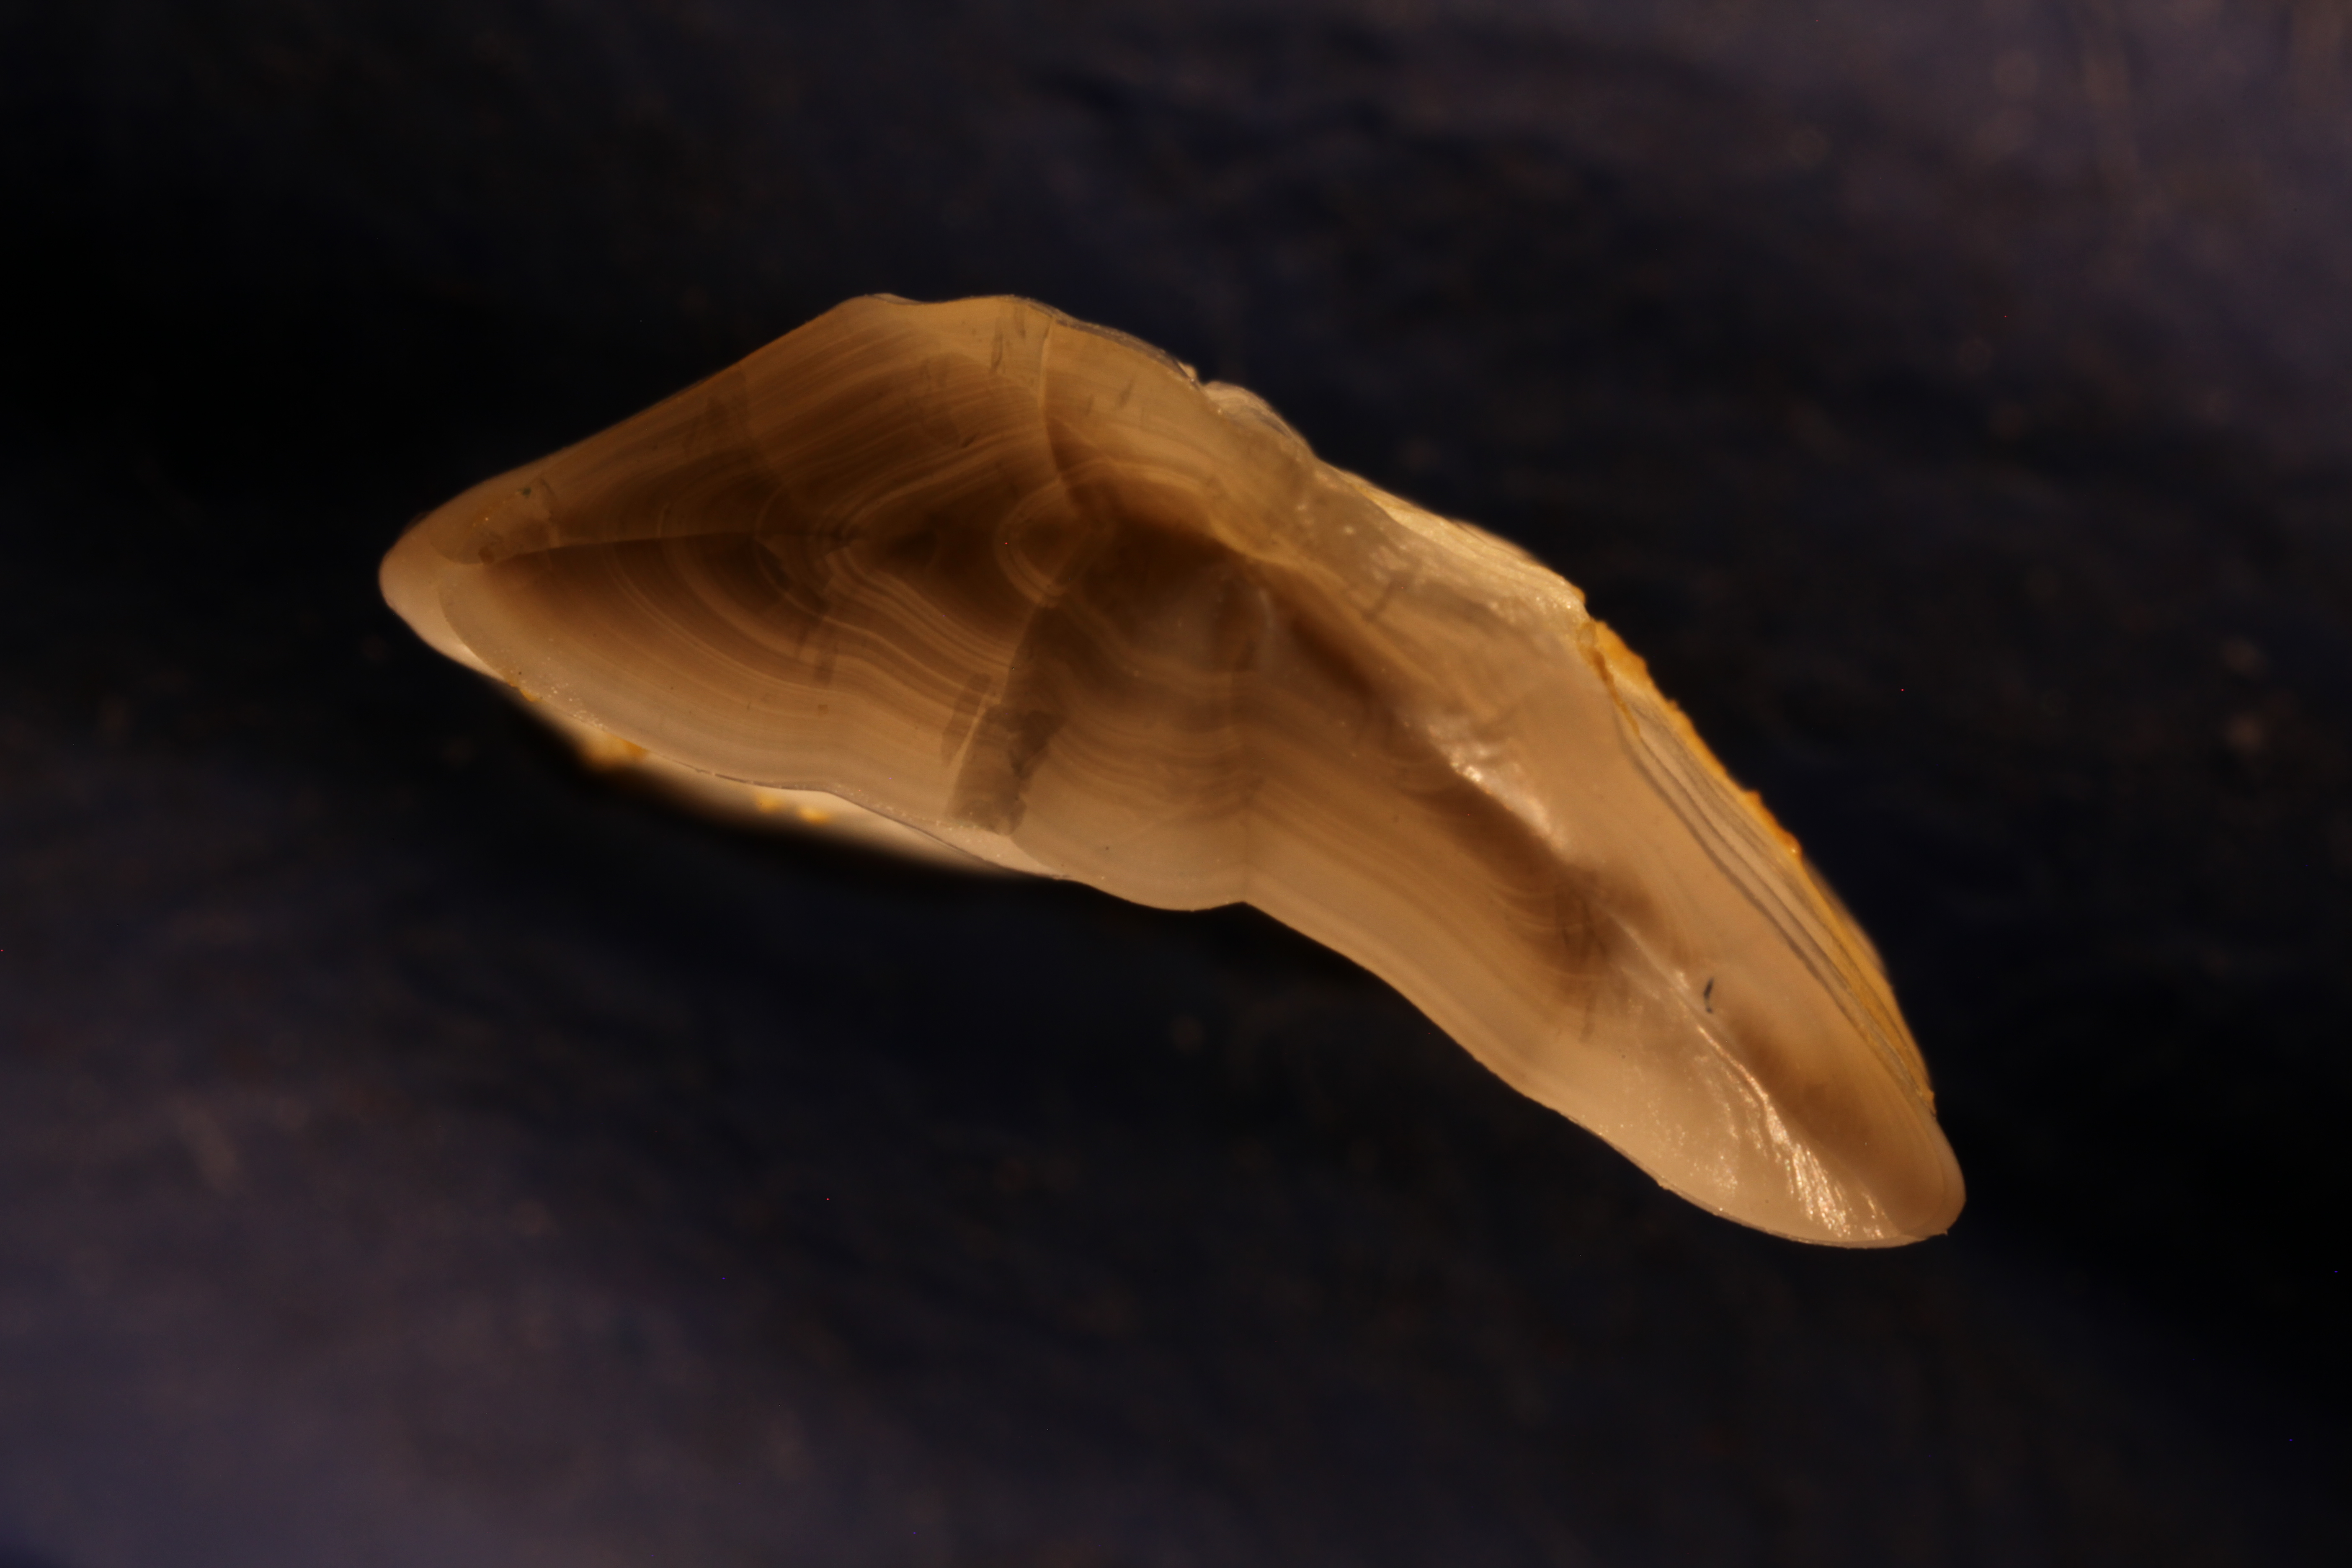
\includegraphics[scale=0.015]{otolith/IMG_0457_2016_70021.JPG}
  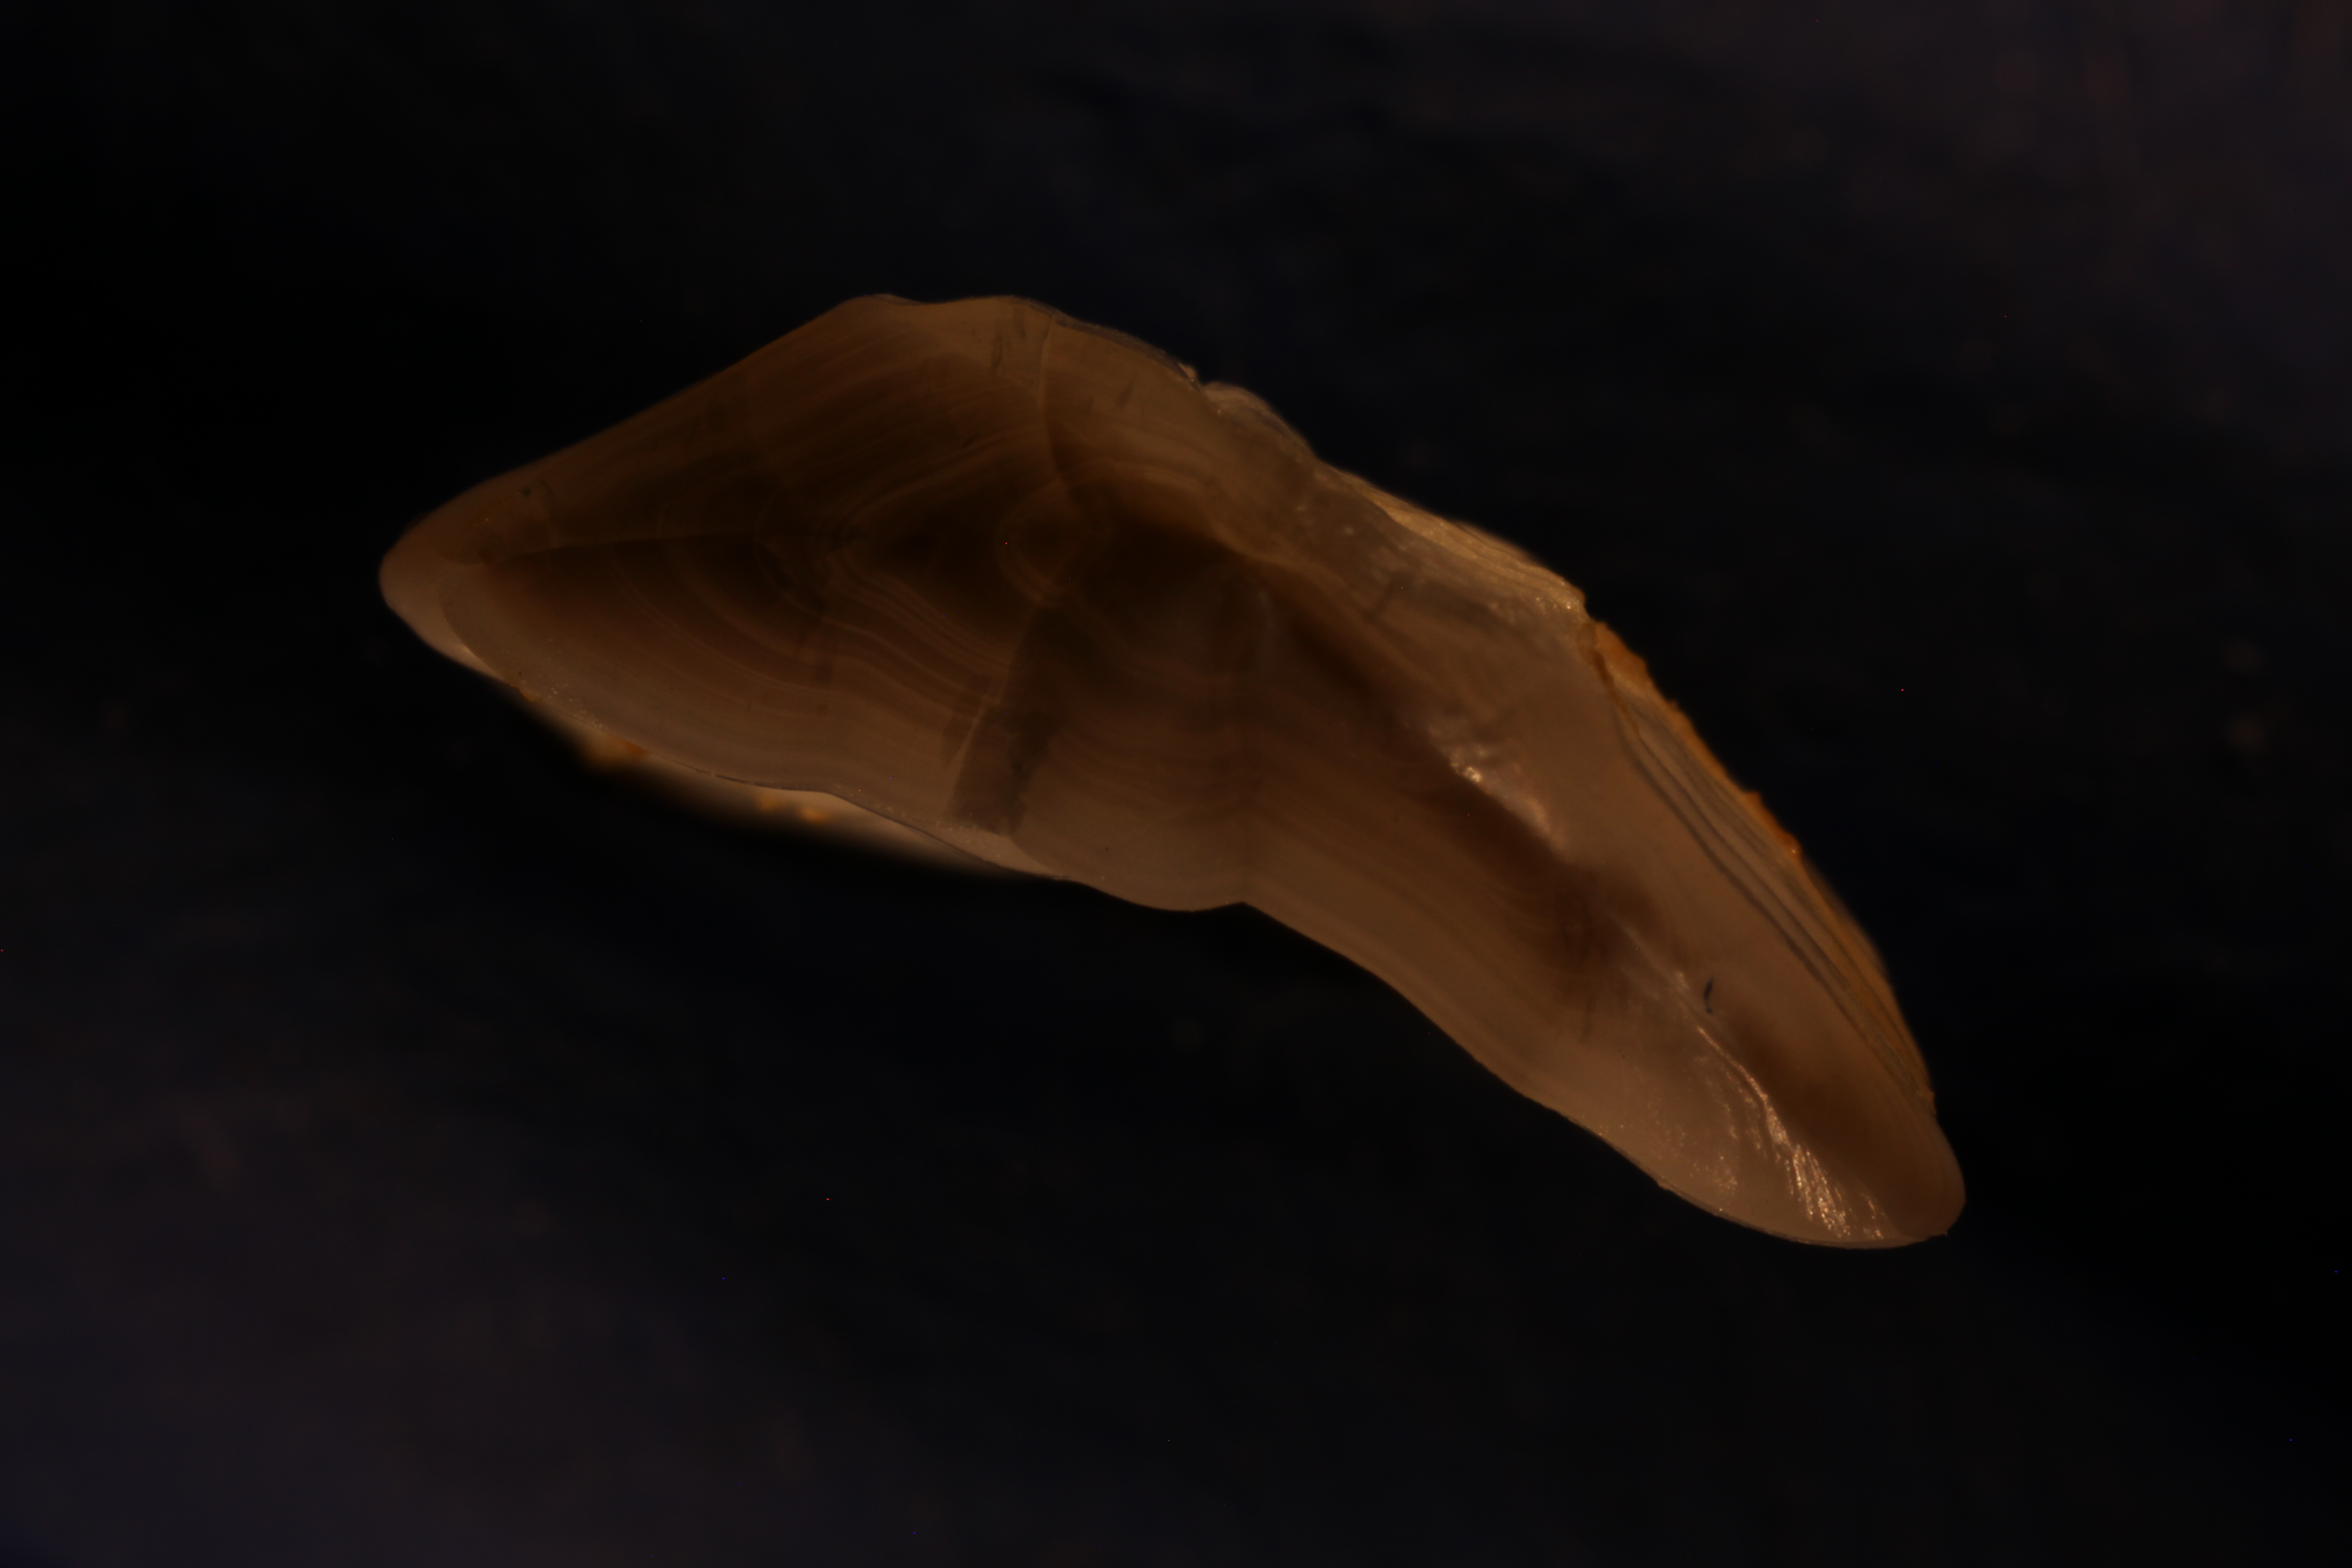
\includegraphics[scale=0.015]{otolith/IMG_0458_2016_70021.JPG}
  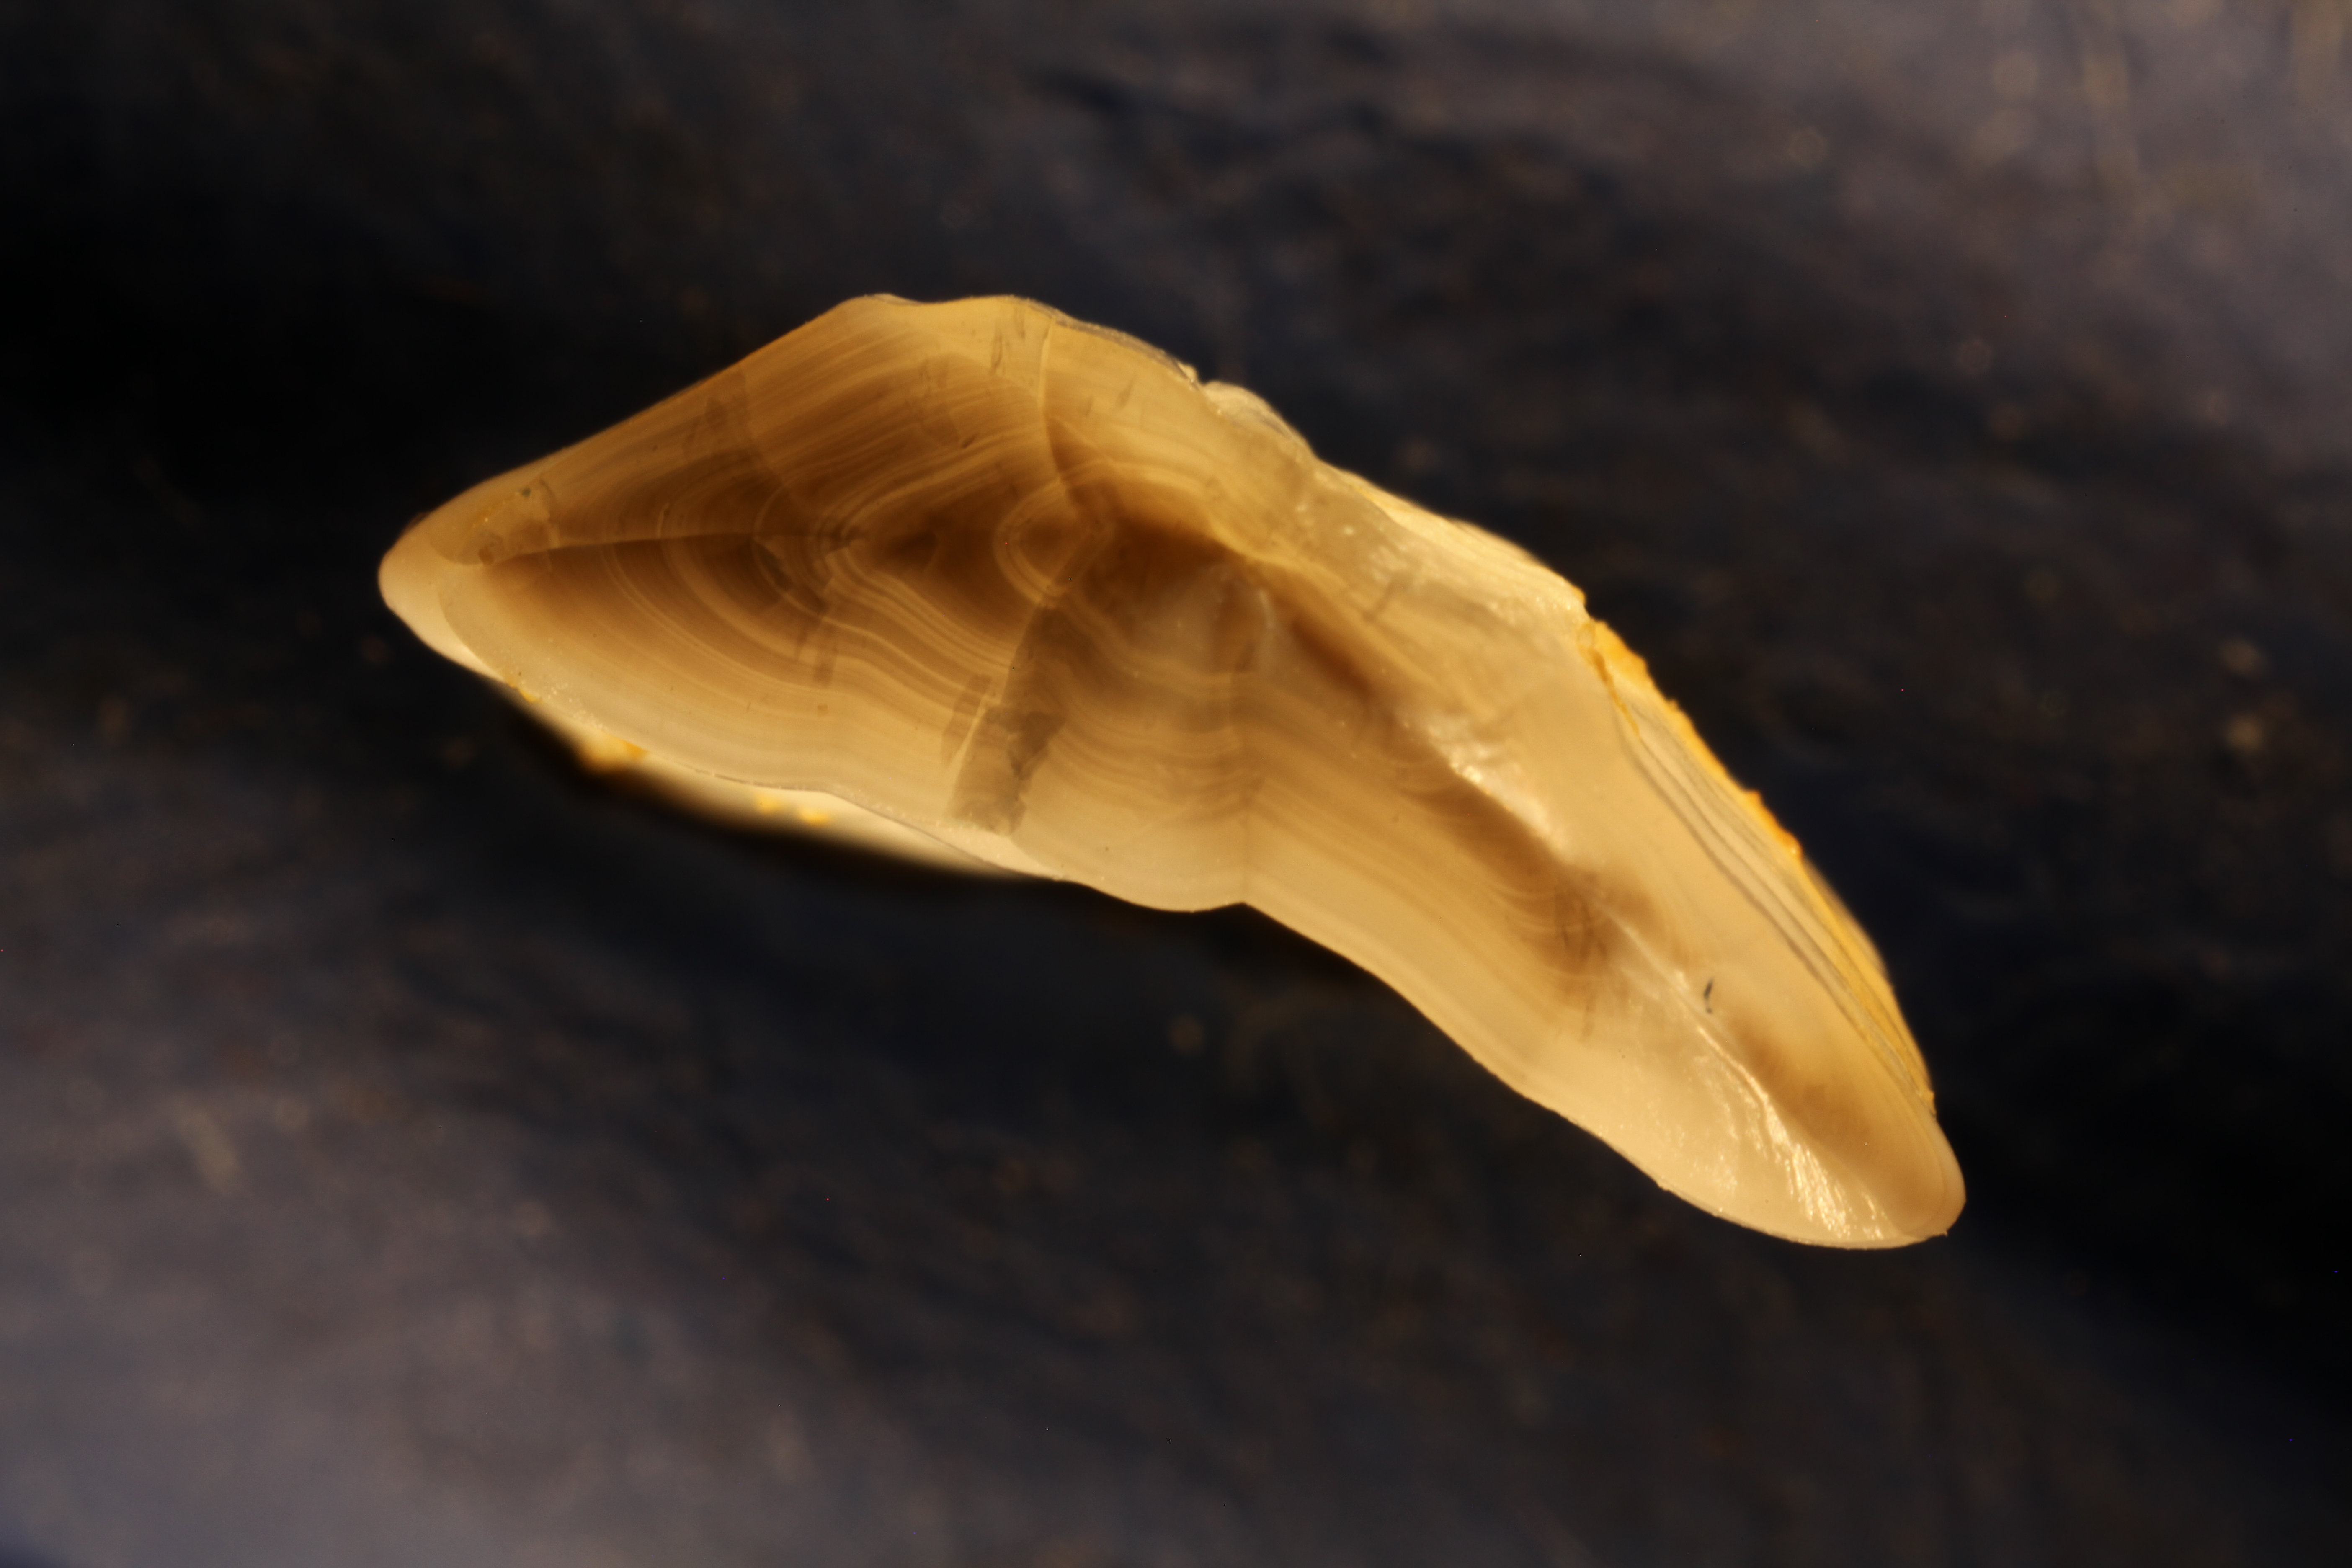
\includegraphics[scale=0.015]{otolith/IMG_0459_2016_70021.JPG} 

  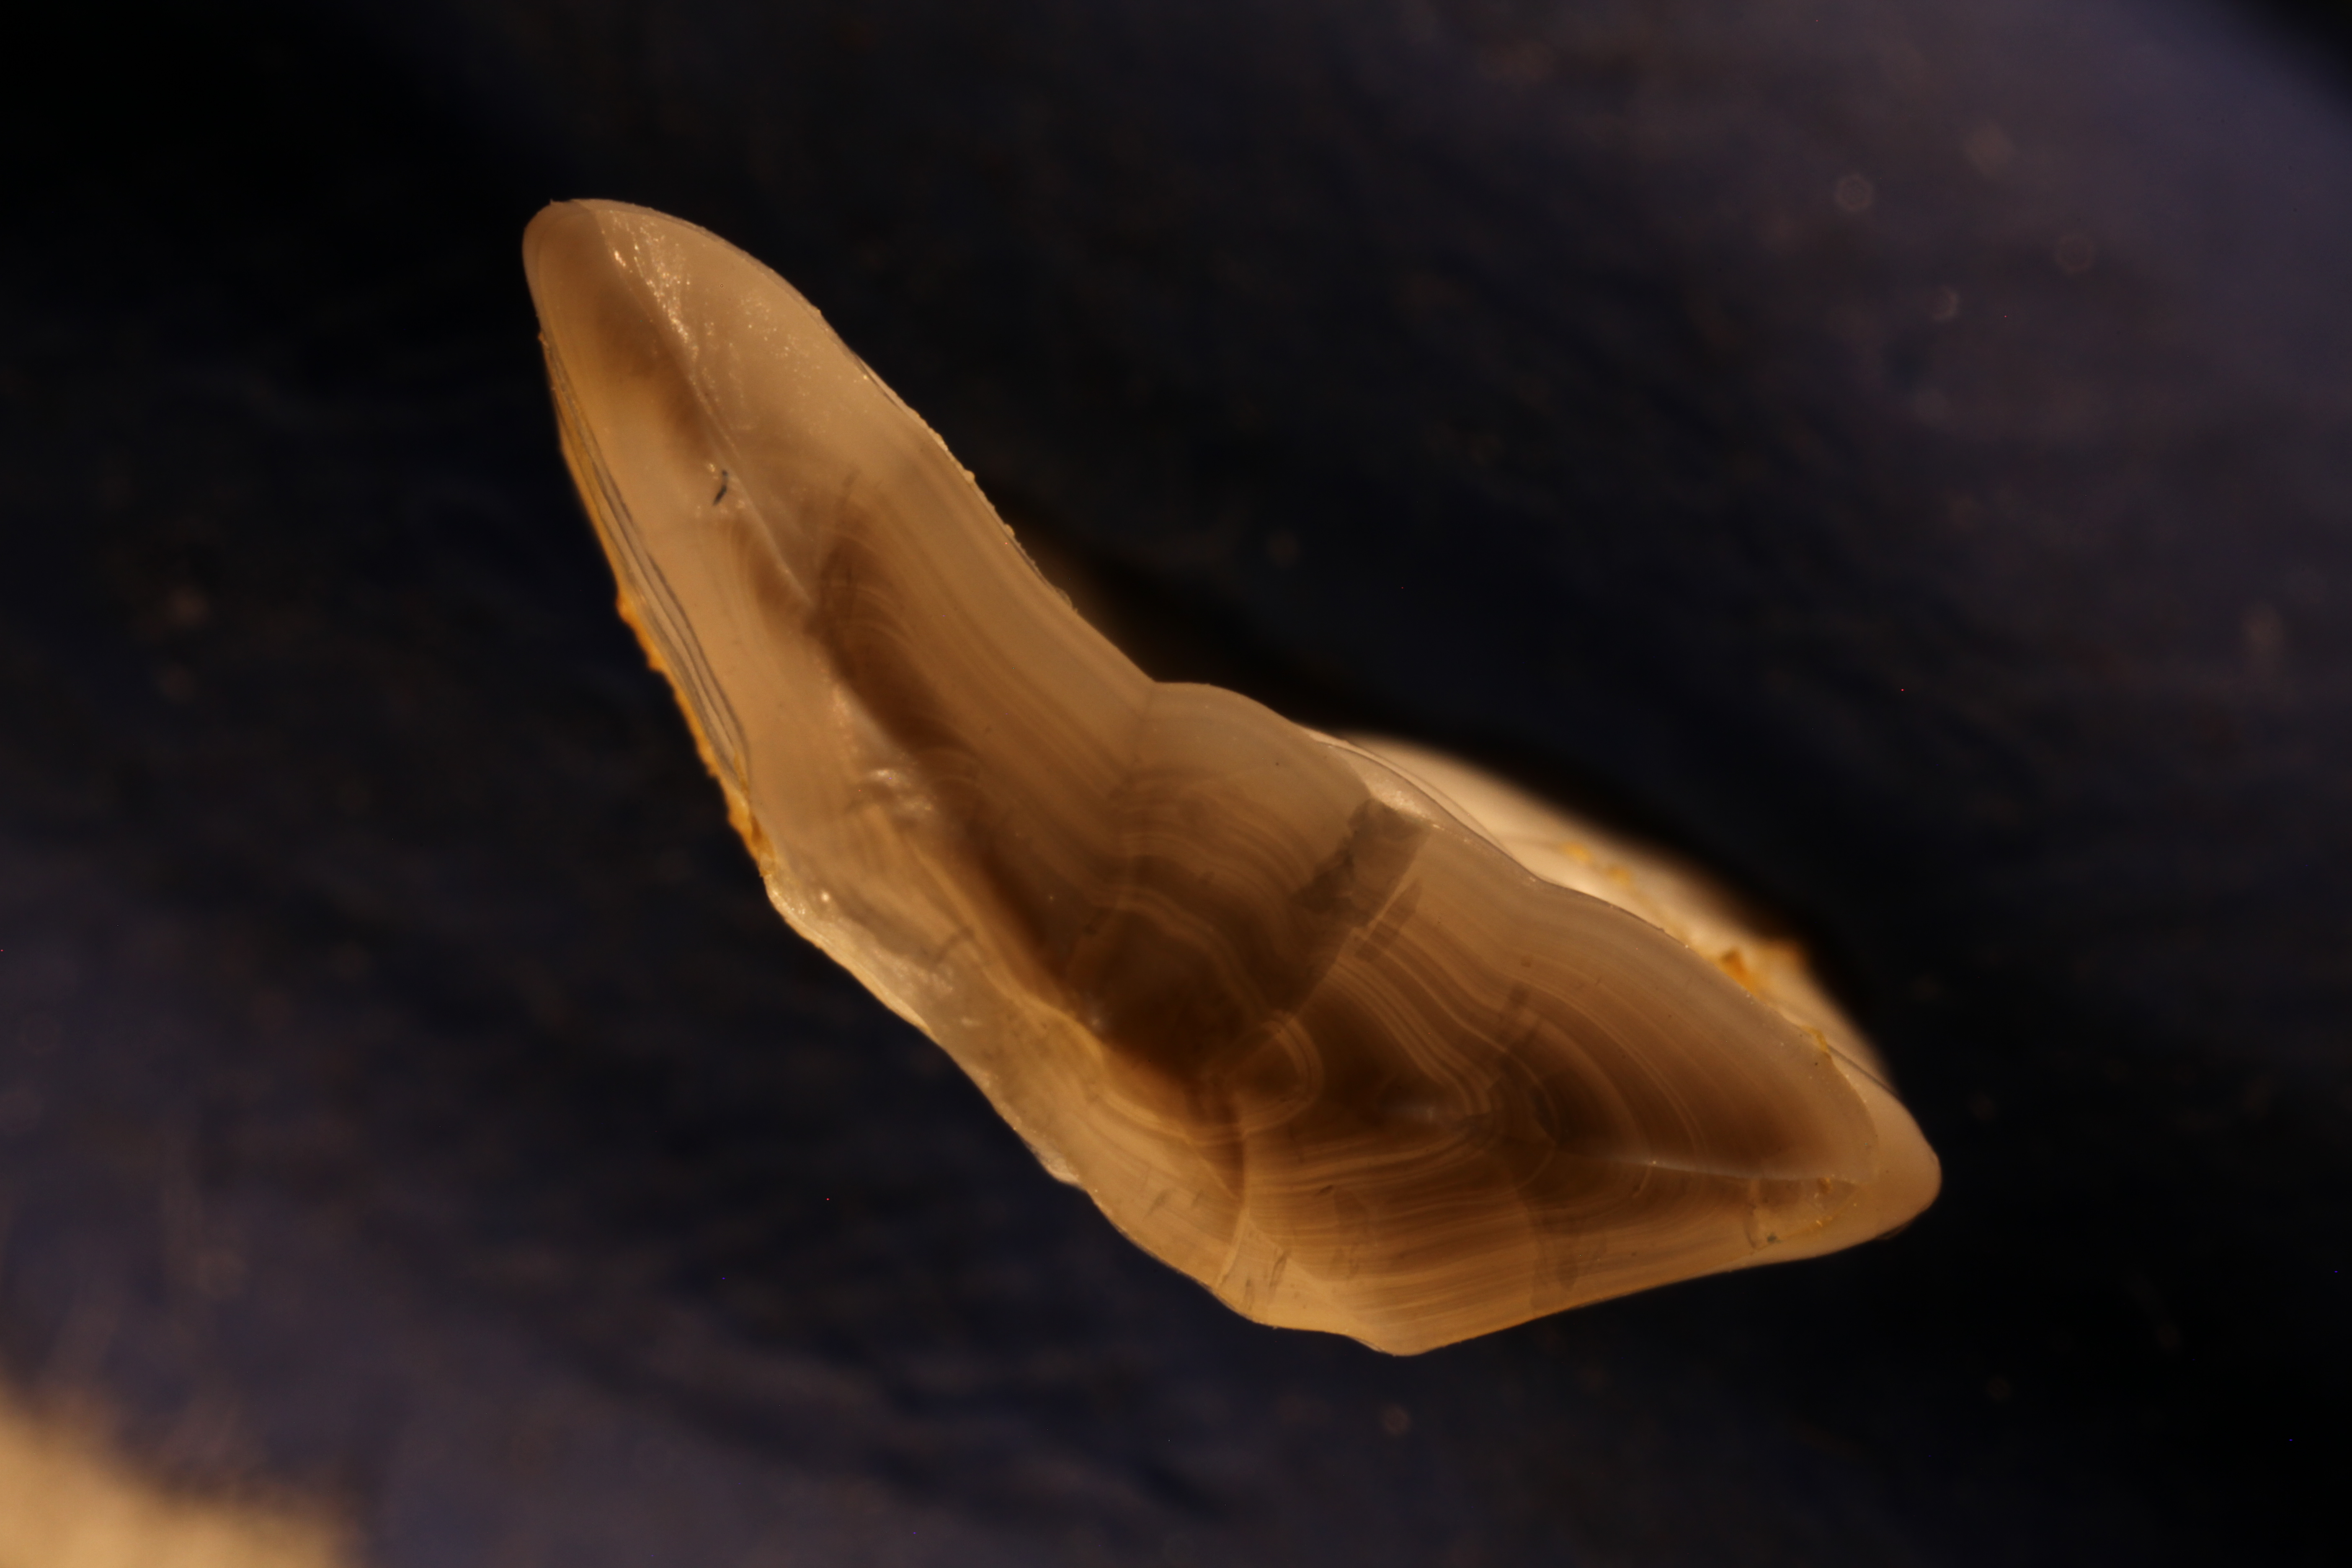
\includegraphics[scale=0.015]{otolith/IMG_0460_2016_70021.JPG}
  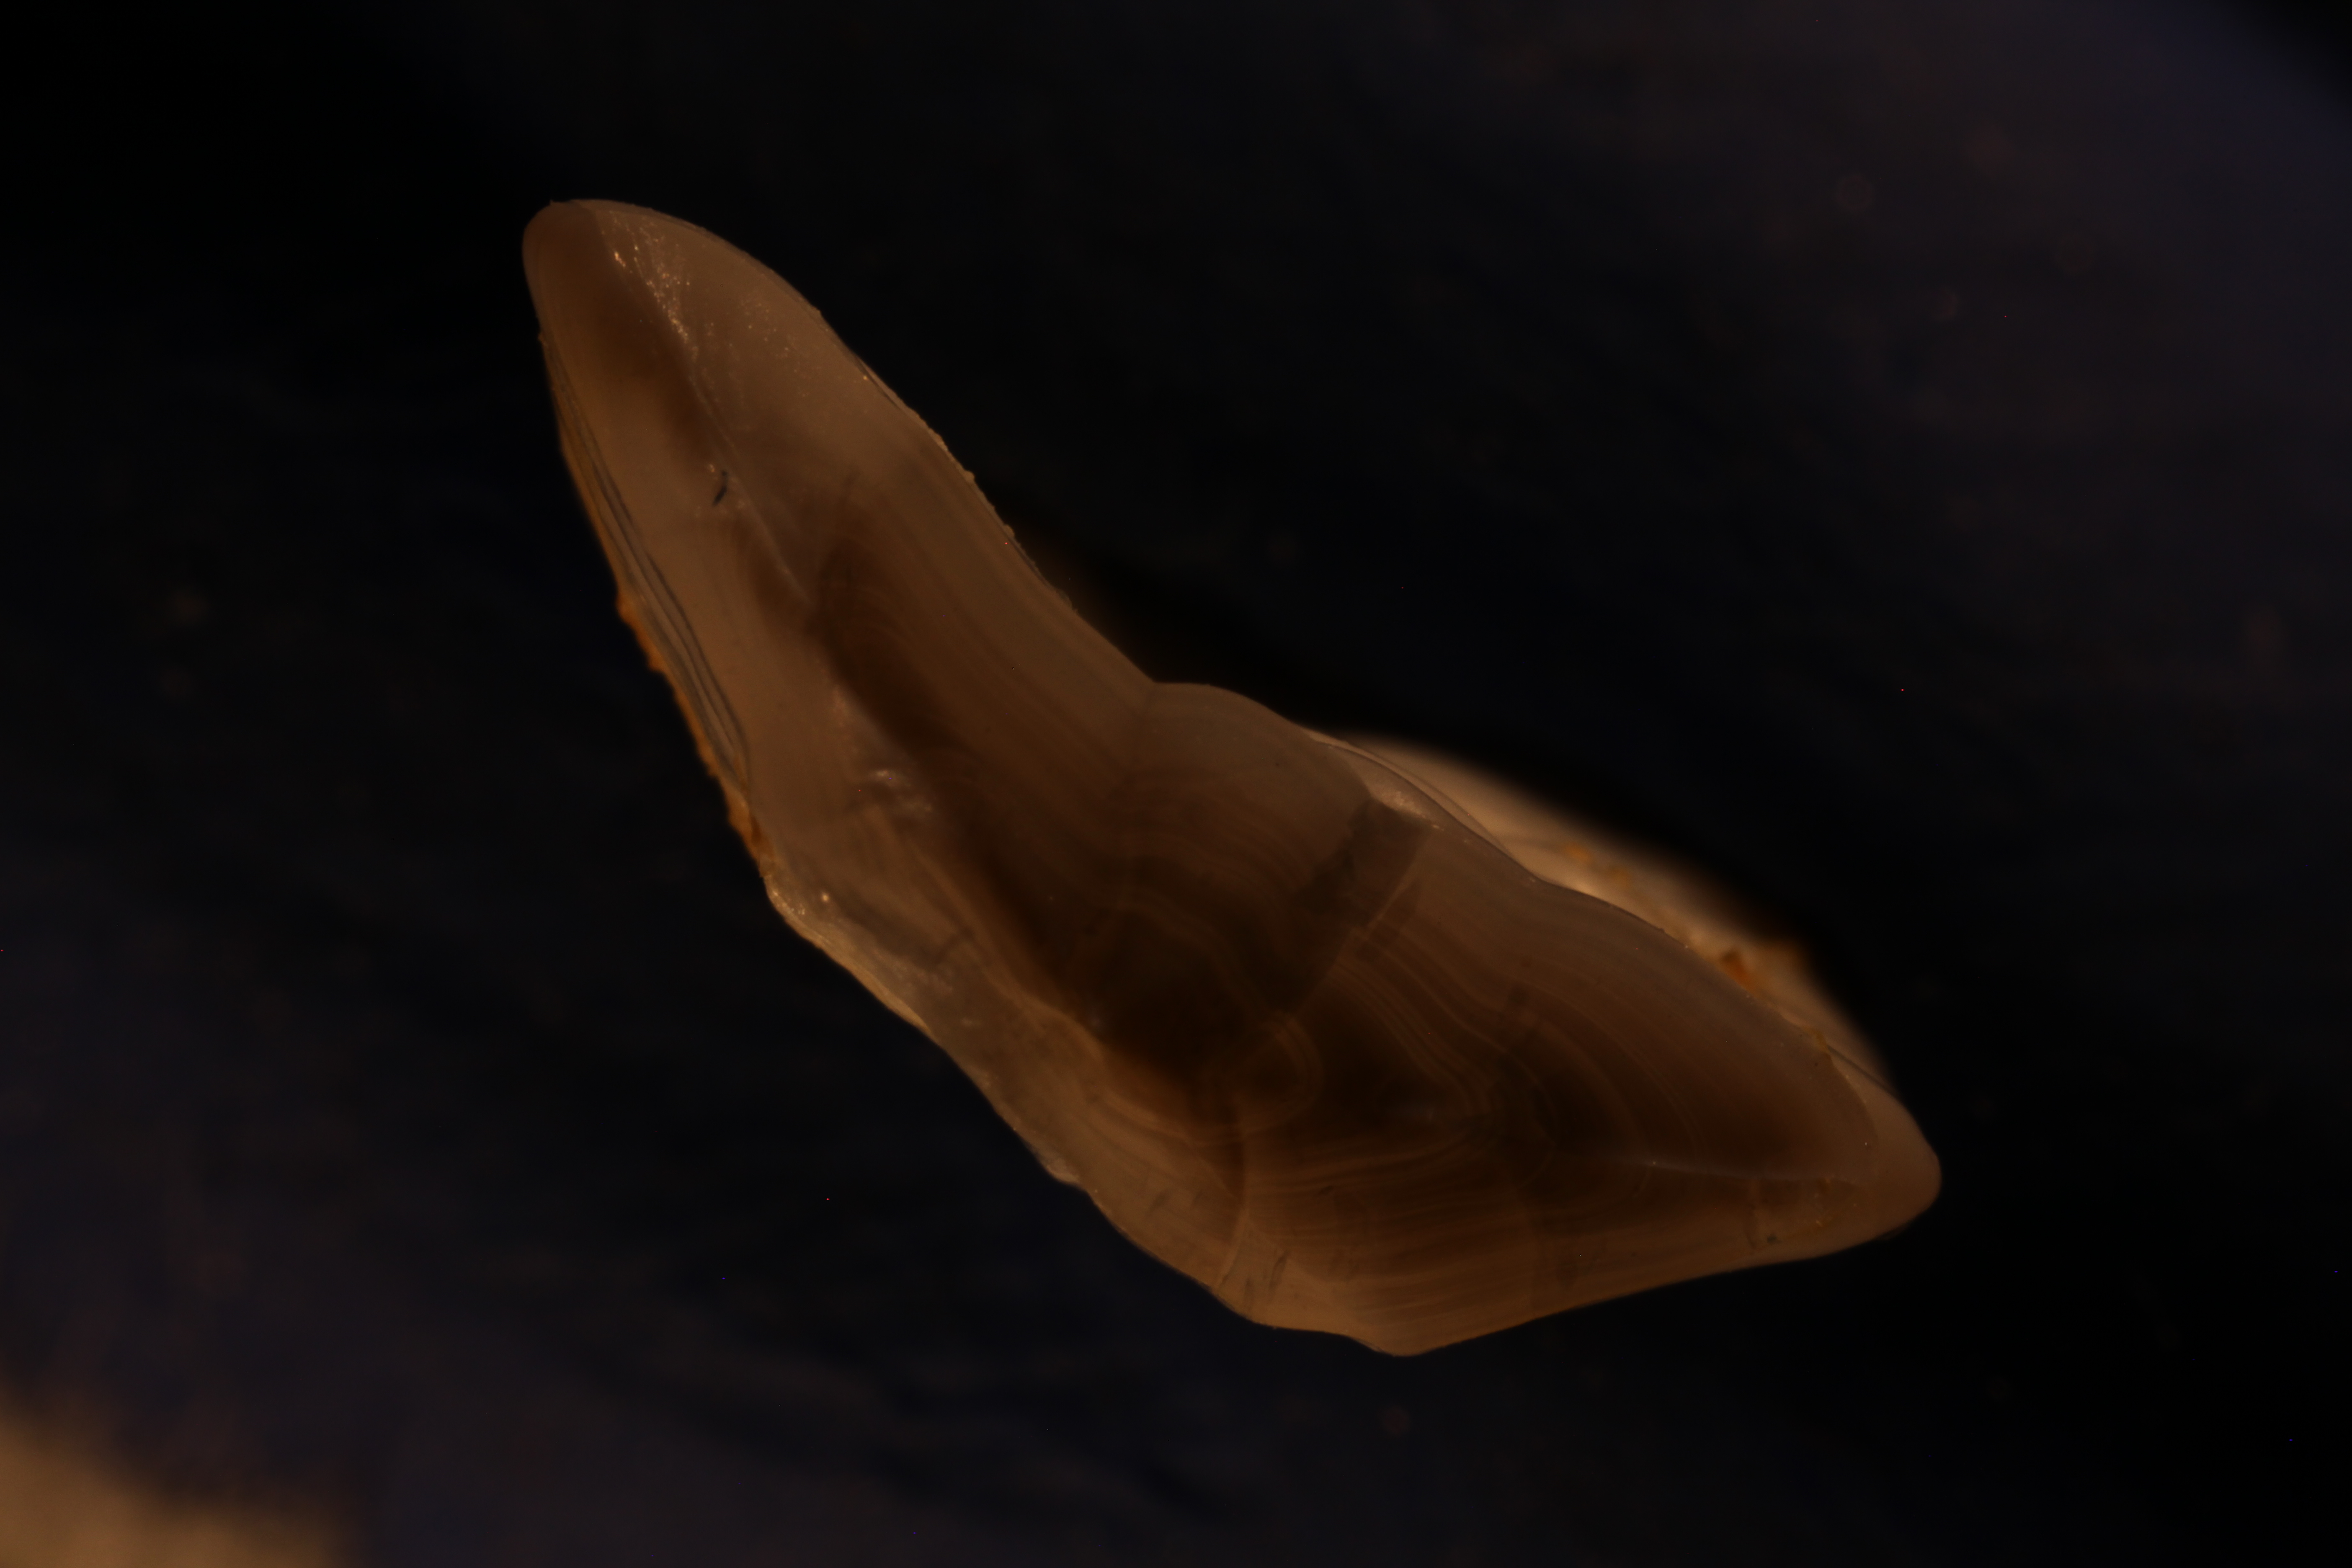
\includegraphics[scale=0.015]{otolith/IMG_0461_2016_70021.JPG}
  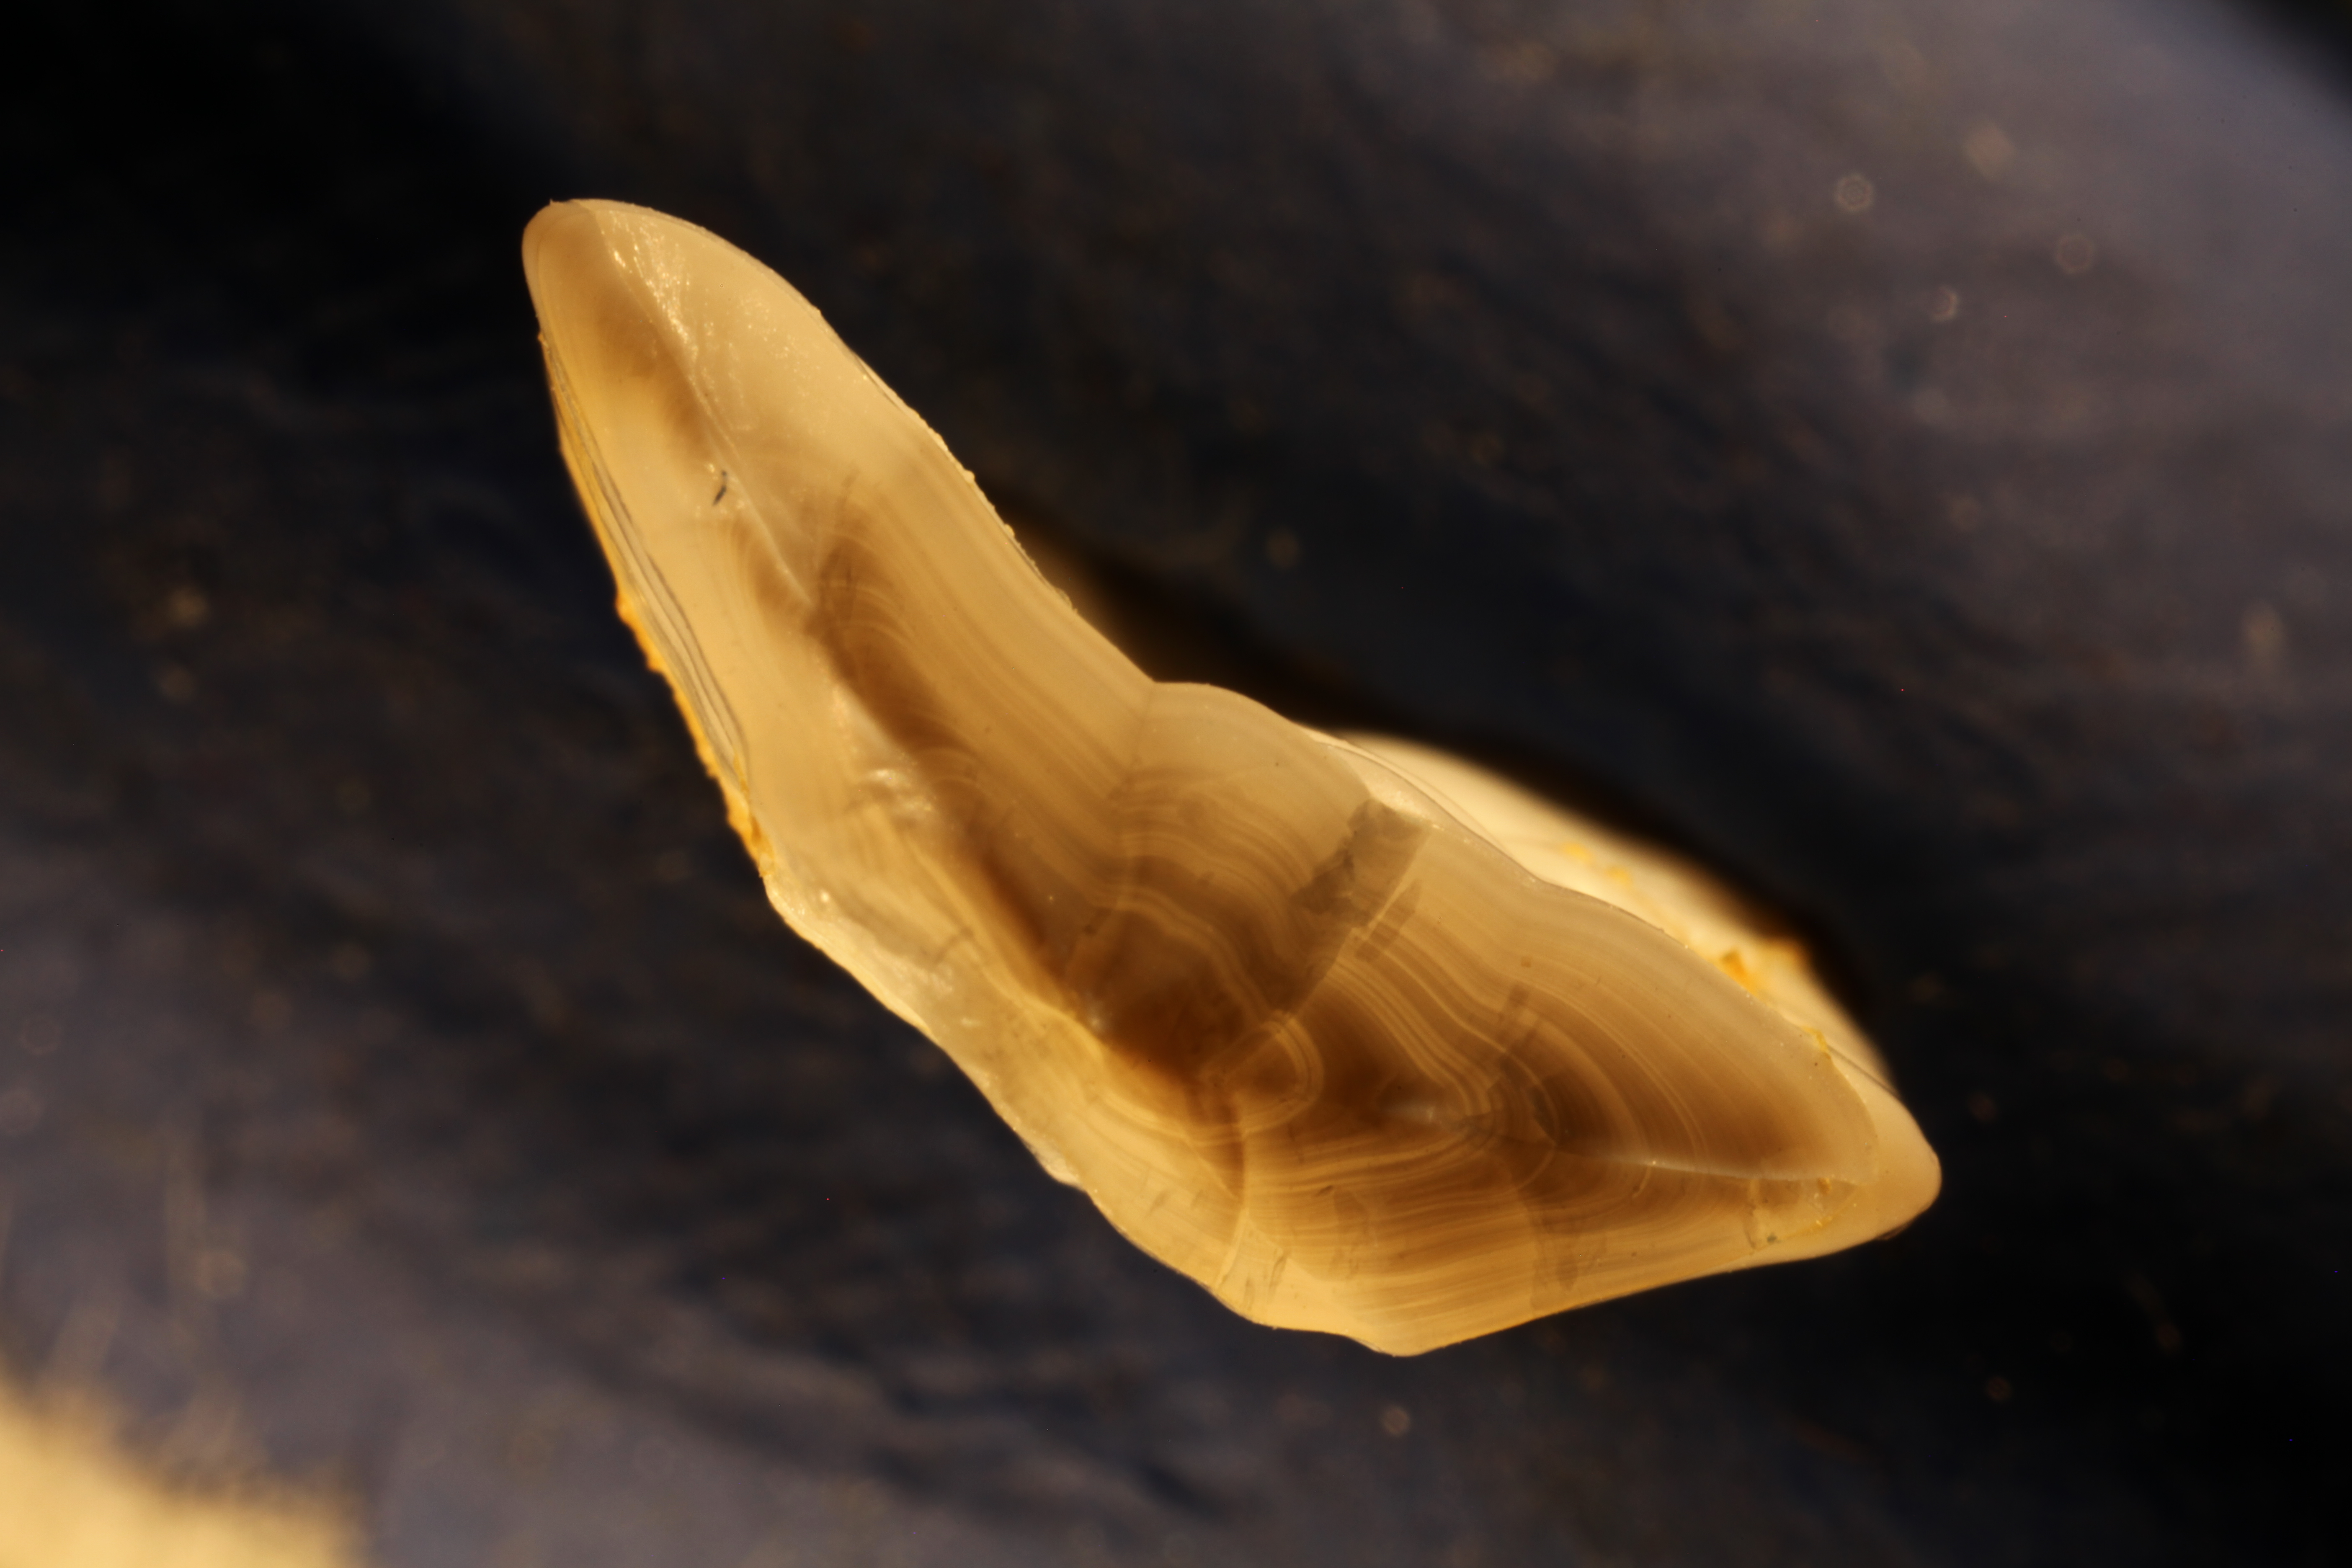
\includegraphics[scale=0.015]{otolith/IMG_0462_2016_70021.JPG}
  
  \label{marker1}
\end{figure}

The images is of size 3744 x 5616 which are re-scaled for training to between 384x384 to 512x512. The image light exposure varies depending on light condition outside, and are stored in the property 'ExposureTime' of the JPG file. Typically the exposure order is middle, dark, or light then a rotation of 180 degrees, and then middle, light, dark again. But the order might change, and
the given order is recovered by reading the metadata property of the jpeg and sorting the exposure time.

The otoliths are prepared for imaging by breaking them.
The process also involves a camera setup, a folder structure referencing 
age, survey and station number, lighting setup, mounting of camera, and 
finally camera capture. More information about this process
can be found in \Mycite{codOtolithsMyers}


\begin{figure}[h!]
  \centering
  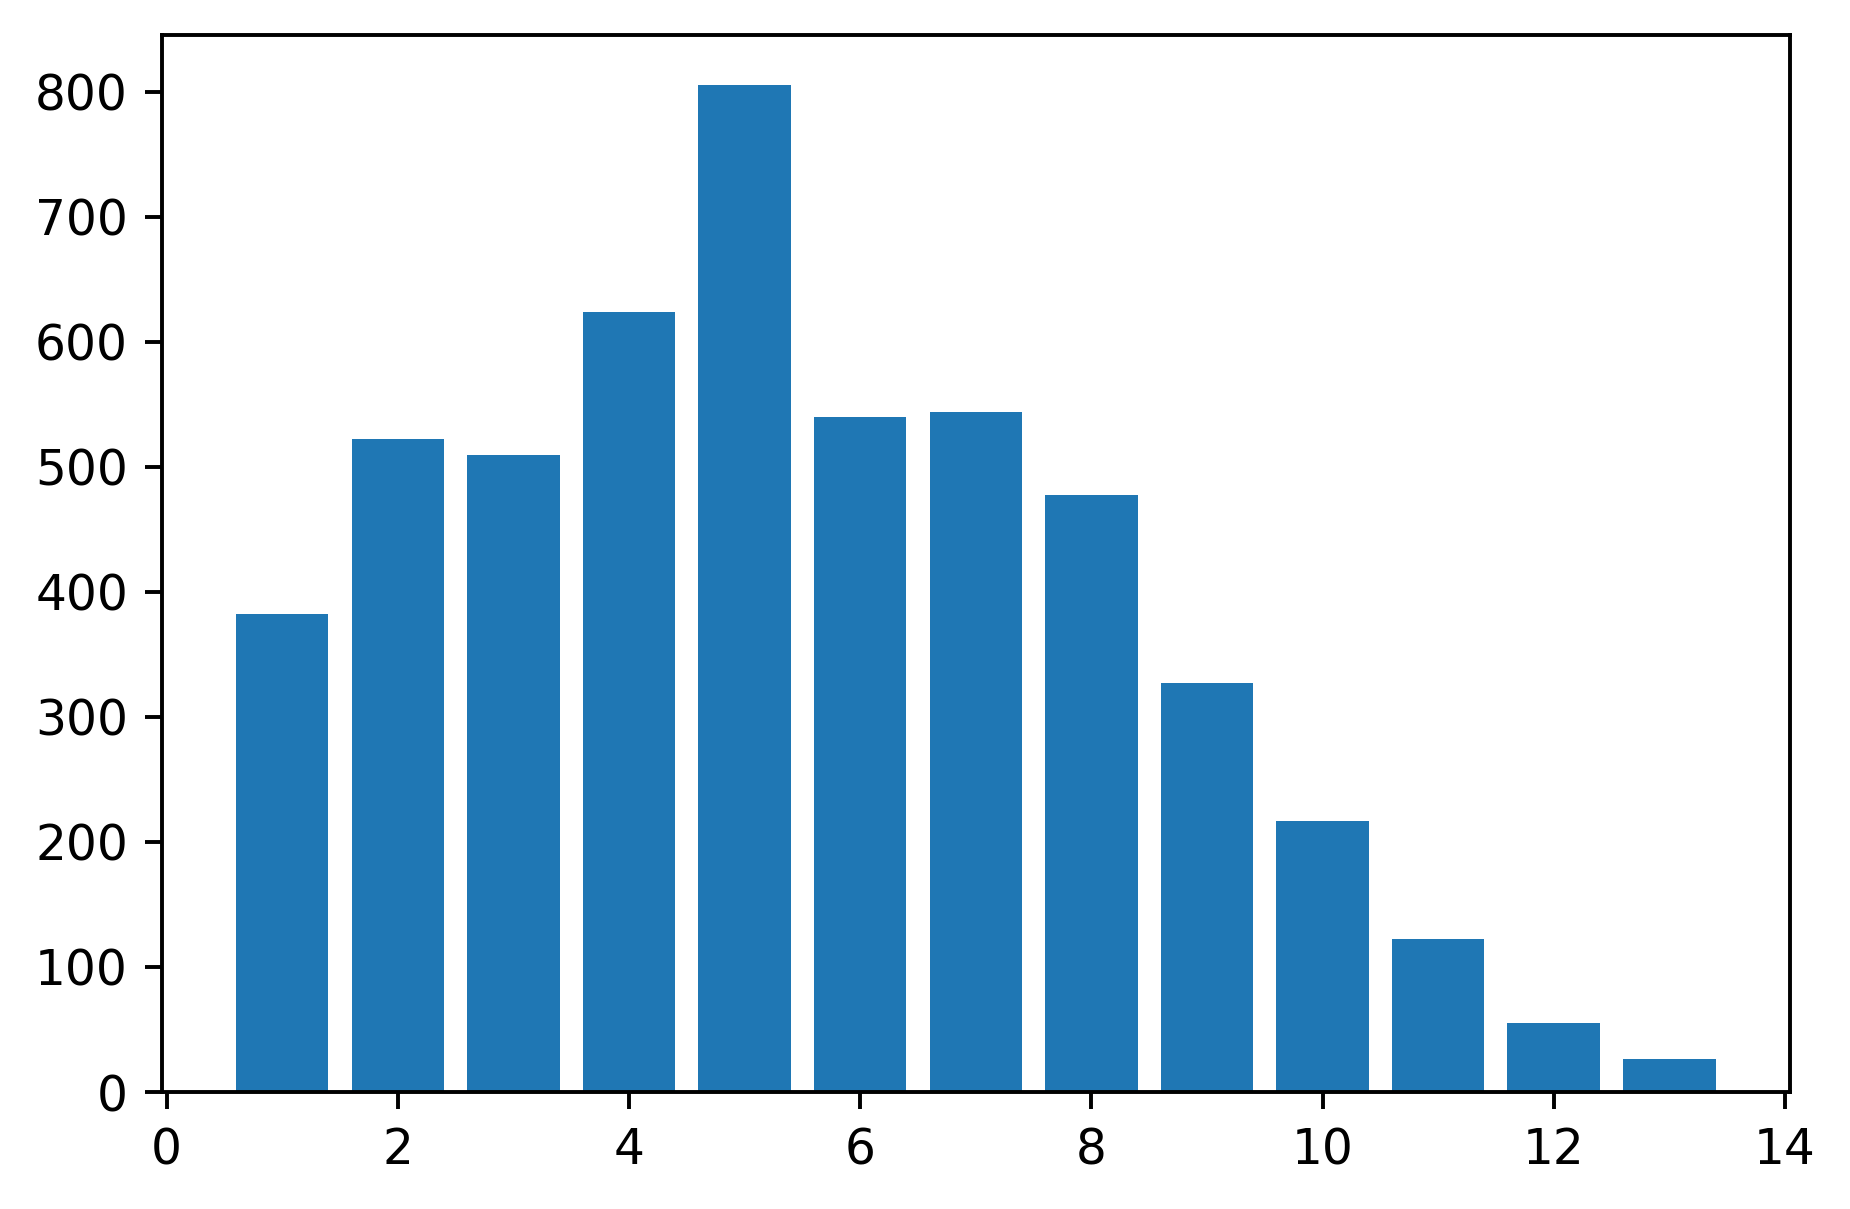
\includegraphics[scale=0.60]{distribution/age_distribution.png}
  \caption{Age distribution of all 5150 images}
\end{figure}

\begin{figure}[h!]
  \centering
  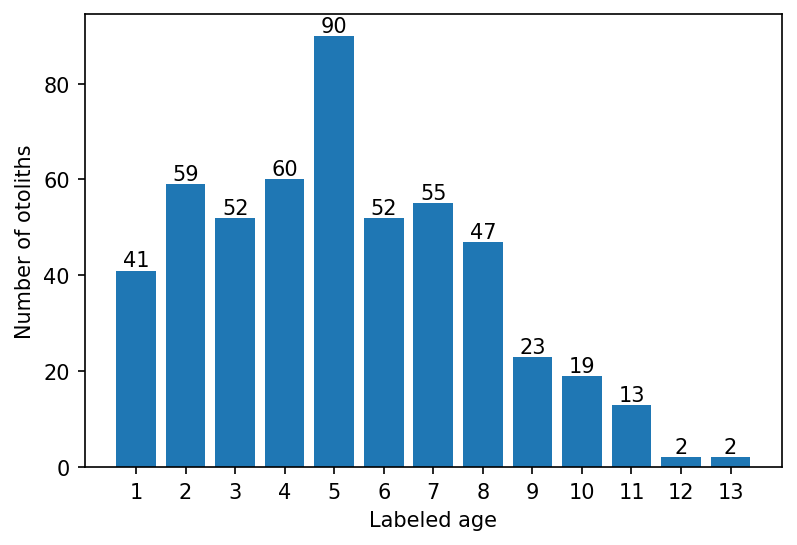
\includegraphics[scale=0.60]{distribution/age_distribution_test.png}
  \caption{Age distribution of 515 images from the test set}
\end{figure}

\subsection*{Preprocessing and augmentation}

To create a large data set with millions of images needed to evaluate the models, we use image augmentation. Image augmentation has made it possible to do deep CNN training on smaller data sets \citep{krizhevsky2012imagenet}. By using this technique it is possible to create millions of training images.

The augmentation methods that we use are rotation by 0 to 360 degrees, and reflection by the vertical (or horizontal) axis. This can be done without loss of information. Also the age reading is agnostic to orientation.

No other augmentation techniques was used like  cropping, shifting or shearing as it can result in loss of age structure information.

The augmented data set can produce 360*2*5150 = 3.708.000 possible images.
Depending on the augmentation factor and the number of images in a training cycle, the model will likely never see the same image twice.
% \citep{boureau2010theoretical} 

The data has been split into train and test-set with 10 \% test-set, 9 \% validation
and 81 \% training-set. Training has been done on the 90 \% of the data set, 4635 images, with 10-fold split producing 10 models. While predictions are made on the 515 images in the test set. The final prediction is
an ensemble prediction on the given model recorded as the expectation on predictions on the test set from the 10 models. 

\begin{figure}[h!]
  \caption{Otolith from 2013, read age: 6. With light exposure: medium, low, high, 
  and expectation per channel of the three exposures. }
  \centering
  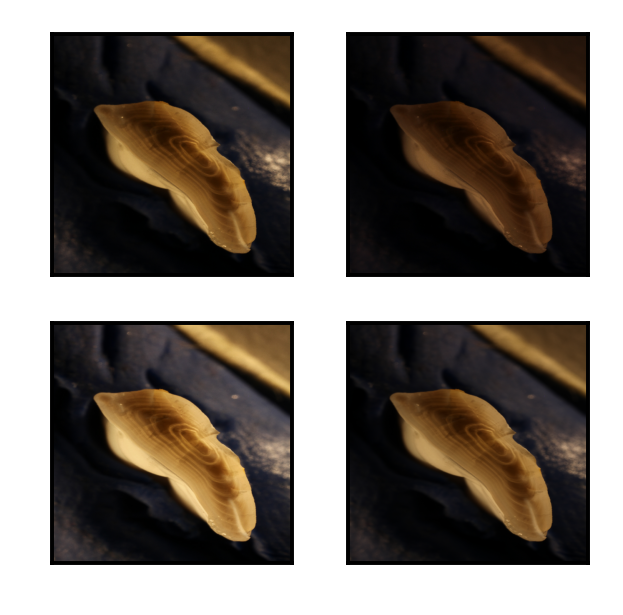
\includegraphics[scale=1.0]{otolith/2013_70174_Nr06_age09_IMG_0031_32_33.png}
  
  \label{marker1}
\end{figure}

\subsection*{Training the Convolutional neural networks}

There are two families of models used, EfficientNet B4-B6 \citep{EfficientNet}   from Tensorflow \citep{abadi2016tensorflow} with a Keras  \citep{keras} implementation plus weights, and a PyTorch \citep{PyTorch}  implementation of EfficientNet V2 medium, Large 
and Xtra-Large \citep{EfficientNetV2} implementation with weights from Timm\citep{rw2019timm}. Weights are ImageNet \citep{deng2009imagenet} weights, which is another prerequisite when working with small data sets, in addition to augmentation. The image size varies between 380 and 528 for EfficientNet Bx, and 384 for EfficientNetV2 size medium, large and xtra-large. While test-set size prediction has been done both on 384 and larger resolutions 480 and 512 as described in the paper. To investigate the image-taking protocol described in \citep{codOtolithsMyers} we have is also training on 9-channel images. Three images are stacked to produce a 9-channel. Using Timm\citep{rw2019timm} the imagenet weights are duplicated on the input layer to accommodate 9 channels. The 3 images used are of dark, medium and light exposure of the first orientation.

EfficientNetV2 has been modified sligtly because the objective is regression as opposed to classification. The output layer of EfficientNetV2 becomes input to a Multi-Layer Perceptron (MLP) of 256 and 32 layers and then to a linear activation function which is the predicted age. More specifically; the 1280 layers output from EfficientNetV2 is input to 256 layer-MLP, then a leakyRelu \citep{DBLP:journals/corr/XuWCL15} then 32 layer-MLP, another leakyRelu, then a linear activation function is the output. This outperformed a linear activation on the 1280 layers from EfficientNetV2, likely because we are doing a regression.

We train and tune EfficientNet B4, B5, B6 \citep{DBLP:journals/corr/abs-1905-11946}, EfficienetNetV2 medium, large \citep{DBLP:journals/corr/abs-1905-11946}, and xl. 
The test results from top models are ensembled to produce the final prediction.

Hyper-parameter tuning is an important step when working with a new dataset and architecture. Some hyper-parameters
that as been tuned are batch size, learning rate, k-fold size, weight decay, step size, number of epochs, early stopping, and
patience. To keep track of all these parameters, a config.json file has been written for each model trained, and 
the exact configuration can be found the the results section of the github page of this project
(https://github.com/emoen/Deep-learning-for-regression-of-cod-otoliths)


\subsection*{Ensemble of ensembles}

As previously mentioned, the results recorded per model is an ensemble of 10 models trained on 10-fold split of the
training data set. Typically the ensemble prediction is better than any single fold prediction. Ensembles are better because they improve 
performance. An ensemble can make better predictions and achieve better performance than any single contributing model, just as more
experts will produce higher accuracy in predicting a single otolith.
Robustness; An ensemble reduces the spread or dispersion of the predictions and model performance.
This result can be improved further by taking ensemble predictions of multiple models as prediction on the test set.
We look at all ensembles from tuple predictions consisting of 2 models, which produces an ensemble of 20 models,
to ensemble of all models which produces an ensemble consisting of 210 models. 
By choosing the best model we are over fitting to the test-set, but 
selecting a subset of the best of these ensembles should produce a candidate ensemble
of ensemble which will produce the best prediction on a test-set holdout set.

\subsection*{Evaluation metric}

The primary metric used for training the models is mean squared error (MSE)
while the primary metric used for evaluating the models is Accuracy.
Accuracy is obtained by rounding the floating point number predictions
to nearest integer and comparing the age classification against the true labels.
To reach human level accuracy a score of 85\% or higher is required \citep{ref_needed}.

\section*{Results}

We have conducted a series of experiments on the EfficientNet family of CNNs, 
with different hyper-parameters and on images with light exposures 
from the set light, medium, dark.
Training has been done on the 10-fold cross validation set which produced 10 models.
An ensemble of the best models produced the best accuracy score in 
table \ref{table1} and MSE in table \ref{table1}.
It can be observed that in the efficientNetV1 family,
larger networks has better MSE, while accuracy is more fluctuating.
A similar pattern can be observed for the efficientNetV2 networks.
Howerver it seems like efficientNetV1 is better than V2, unlike
the results observed on ImageNet.

\begin{center}
\begin{table}[hbt!]
\caption{Accuracy by light exposure and CNN architectures}
\begin{tabular}{ |l|c|c|c|c|c|c| }

\hline
MSE:light/CNN & B4 & B5 & B6 & Medium & Large & Xtra Large \\ \hline
min        & 72.8 & 74.4 & 73.4 & 67.0* & - & - \\ 
medium     & - & - & 74.4 & 72.4 & 71.8 & - \\ 
max        & - & - & - & - & - & - \\ 
9 channels & - & - & - & - & 71.7 & - \\ 
\hline
\label{table1}
\end{tabular}
\end{table}
\end{center}

\begin{center}
\begin{table}[hbt!]
\caption{MSE by light exposure and CNN architectures}
\begin{tabular}{ |l|c|c|c|c|c|c| }

\hline
ACC:light/CNN & B4 & B5 & B6 & Medium & Large & Xtra Large \\ \hline
min        & .277 & .277 & .272 & .331* & - & - \\ 
medium     & - & - & .262 & .292 & .280 & - \\ 
max        & - & - & - & - & - & - \\ 
9 channels & - & - & - & - & .281 & - \\ 
\hline
\label{table2}
\end{tabular}
\end{table}
\end{center}


\begin{figure}[h!]
  \centering
  \begin{minipage}[b]{1.0\textwidth}
  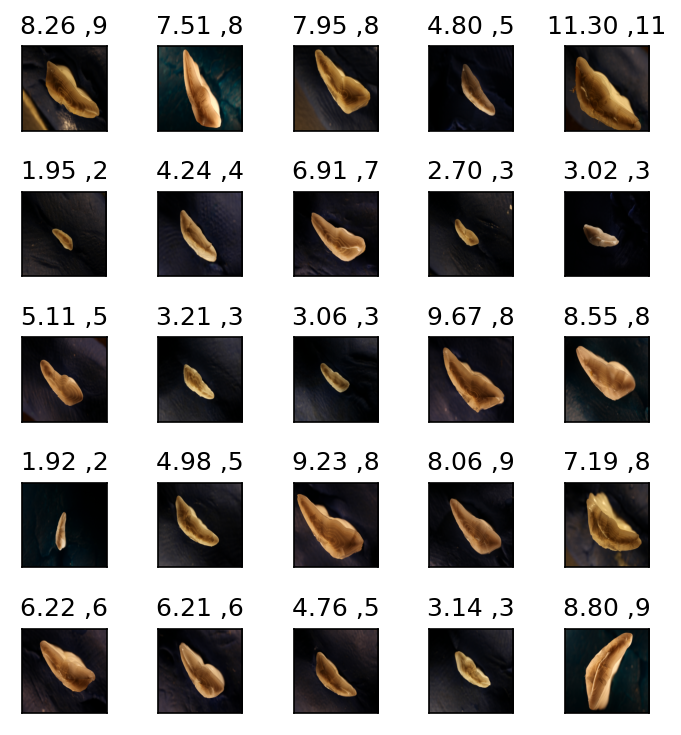
\includegraphics[scale=0.75]{results/fold_prediction_V2_m.png}
    \caption{Sample of 25 predictions on a fold of training on EfficientNetV2 size medium with minimum light exposure, left number is prediction,
    and right number is age read
    
    }
   \label{marker3}
  \end{minipage}
  \hfill
\end{figure}

We compare the 10 fold prediction accuracy of all the models in a box plot in
figure \ref{marker4}, and for MSE in \ref{marker5}. The metric for
each of the 10 folds are given by the box plot, and the red line 
is the ensemble accuracy or MSE. The ensemble metric is either better than 
all the folds or in the upper quantile.

\begin{figure}[h!]
  \centering
  \begin{minipage}[b]{0.49\textwidth}
  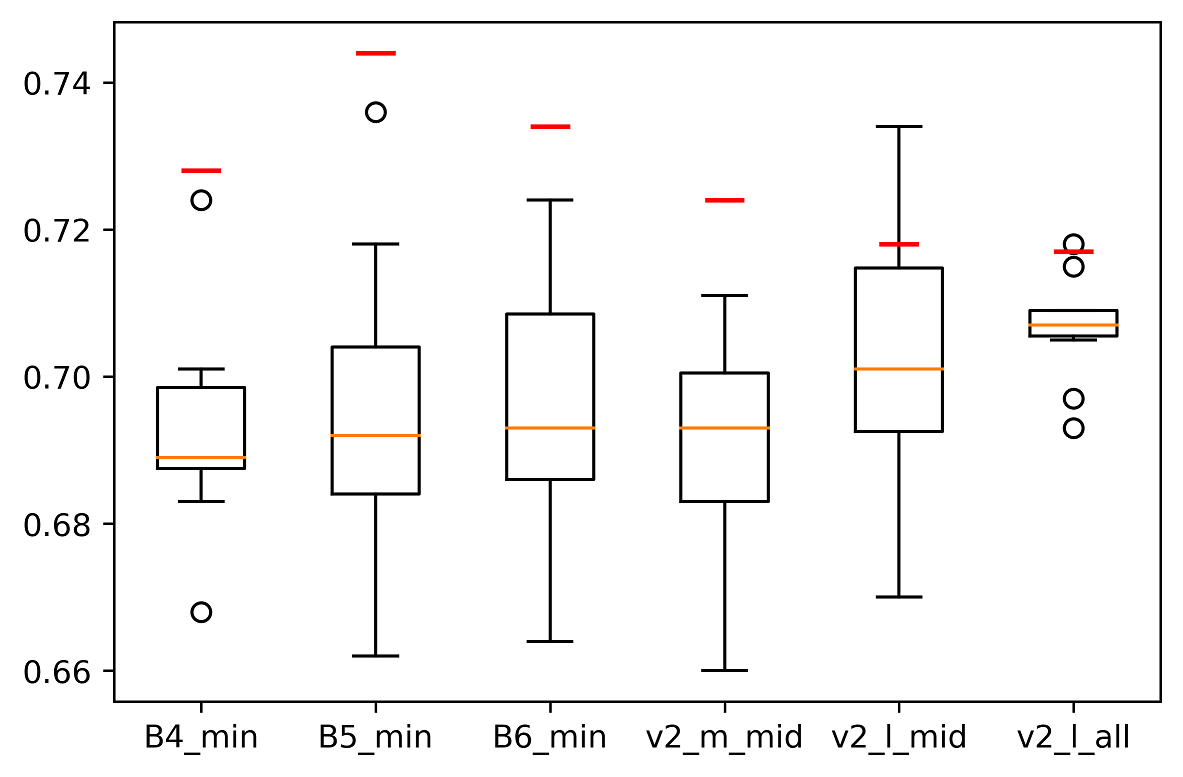
\includegraphics[scale=0.2]{results/box_plot_models_acc.png}
    \caption{Accuracy score of 5 models and red line is ensemble prediction accuracy}
   \label{marker4}
  \end{minipage}
  \hfill
\end{figure}

\begin{figure}[h!]
  \centering
  \begin{minipage}[b]{0.49\textwidth}
  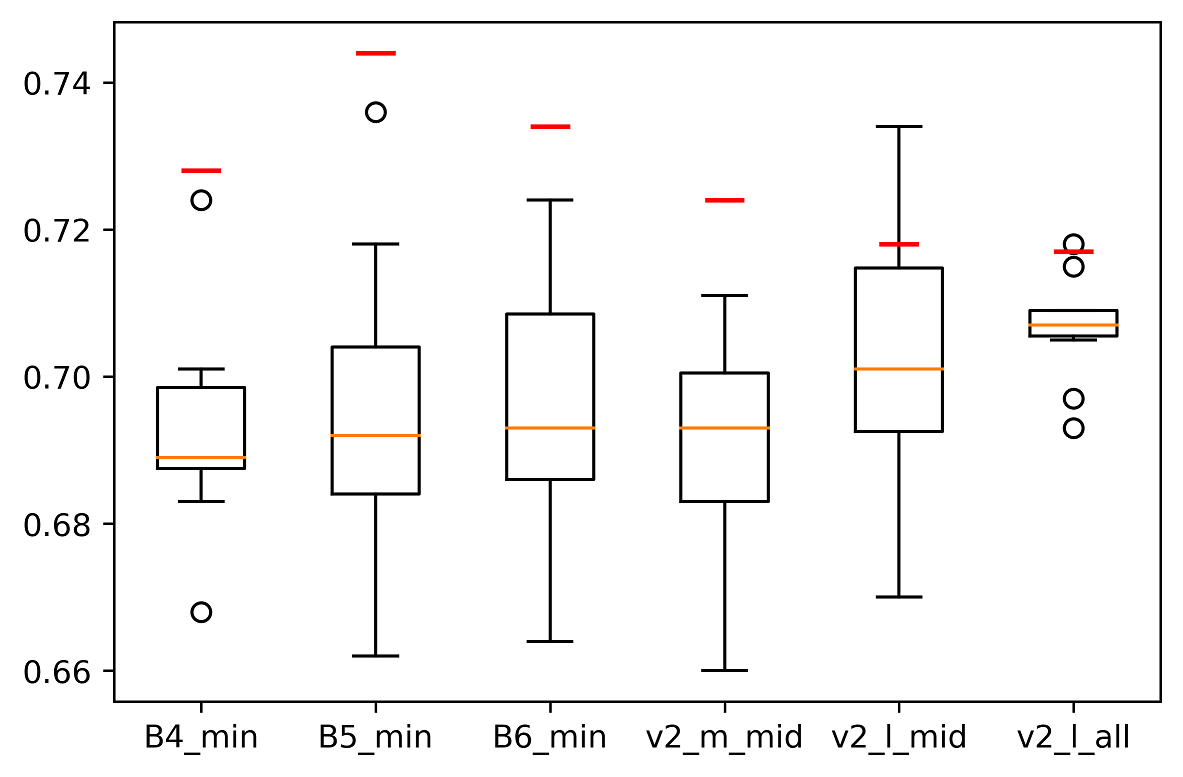
\includegraphics[scale=0.2]{results/box_plot_models_acc.png}
    \caption{MSE score of 5 models and red line is ensemble prediction MSE}
   \label{marker5}
  \end{minipage}
  \hfill
\end{figure}

By comparing the models on MSE we can see that larger models are better, e.g B6 has 
higher mean than B5 and B4, and large is better than medium. 
We also see that the EfficientNetV2 networks has higher mean than mean than the
first generation EfficientNet. However, this is not true for the ensemble
predictions (red line) nor for the mean or ensemble mean of the accuracy.
We can also see that the effect of adding 3 images - 9 channels on the
model is that the variance is reduced.

The box-plots are produced from the fold metrics:
\begin{table}[!ht]
    \caption{MSE per CNN and per fold}
    \centering
    \begin{tabular}{|l|l|l|l|l|l|l|l|l|l|l|l|l|}
    \hline
        CNN/fold & 1 & 2 & 3 & 4 & 5 & 6 & 7 & 8 & 9 & 10 & mse \\ \hline
        B4, min & .320 & .318 & .3. & .313 & .322 & .314 & .315 & .316 & .3. & .3. & .277 \\ \hline
        B4, middle & ~ & ~ & ~ & ~ & ~ & ~ & ~ & ~ & ~ & ~ & ~ \\ \hline
        B4, max & ~ & ~ & ~ & ~ & ~ & ~ & ~ & ~ & ~ & ~ & ~ \\ \hline
        B5, min & .324 & .322 & .325 & .336 & .291 & .314 & .320 & .331 & .33 & .317 & .277 \\ \hline
        B5, middle & ~ & ~ & ~ & ~ & ~ & ~ & ~ & ~ & ~ & ~ & ~ \\ \hline
        B5, max & ~ & ~ & ~ & ~ & ~ & ~ & ~ & ~ & ~ & ~ & ~ \\ \hline
        B6, min & .325 & .329 & .334 & .293 & .312 & .290 & .320 & .3. & .276 & .3. & .272 \\ \hline
        B6, middle & .323 & .3. & .312 & .268 & .294 & .266 & .3. & .311 & .278 & .289 & .262 \\ \hline
        B6, max & ~ & ~ & ~ & ~ & ~ & ~ & ~ & ~ & ~ & ~ & ~ \\ \hline
        medium, min & ~ & ~ & ~ & ~ & ~ & ~ & ~ & ~ & ~ & ~ & ~ \\ \hline
        med., mid. & .321 & .377 & .332 & .285 & .285 & .325 & .311 & .348 & .295 & .373 & .292 \\ \hline
        medium, max & ~ & ~ & ~ & ~ & ~ & ~ & ~ & ~ & ~ & ~ & ~ \\ \hline
        medium, all & ~ & ~ & ~ & ~ & ~ & ~ & ~ & ~ & ~ & ~ & ~ \\ \hline
        large, min & ~ & ~ & ~ & ~ & ~ & ~ & ~ & ~ & ~ & ~ & ~ \\ \hline
        large, middle & .3. & .281 & .299 & .318 & .282 & .3. & .280 & .334 & .3. & .310 & .280 \\ \hline
        large, max & ~ & ~ & ~ & ~ & ~ & ~ & ~ & ~ & ~ & ~ & ~ \\ \hline
        large, all & .292 & .289 & .289 & .326 & .3. & .327 & .283 & .30 & .335 & .295 & .281 \\ \hline
        xl, min & ~ & ~ & ~ & ~ & ~ & ~ & ~ & ~ & ~ & ~ & ~ \\ \hline
        xl, middle & ~ & ~ & ~ & ~ & ~ & ~ & ~ & ~ & ~ & ~ & ~ \\ \hline
        xl, max & ~ & ~ & ~ & ~ & ~ & ~ & ~ & ~ & ~ & ~ & ~ \\ \hline
        xl, all & ~ & ~ & ~ & ~ & ~ & ~ & ~ & ~ & ~ & ~ & ~ \\ \hline
    \end{tabular}
\end{table}

\begin{table}[!ht]
    \centering
    \caption{Accuracy per CNN and per fold}
    \begin{tabular}{|l|l|l|l|l|l|l|l|l|l|l|l|}
    \hline
        CNN/fold & 1 & 2 & 3 & 4 & 5 & 6 & 7 & 8 & 9 & 10 & acc \\ \hline
        B4, min & 69.9 & 68.9 & 68.7 & 68.3 & 68.9 & 70.1 & 69.7 & 66.8 & 68.9 & 72.4 & 72.8 \\ \hline
        B4, middle & ~ & ~ & ~ & ~ & ~ & ~ & ~ & ~ & ~ & ~ & ~ \\ \hline
        B4, max & ~ & ~ & ~ & ~ & ~ & ~ & ~ & ~ & ~ & ~ & ~ \\ \hline
        B5, min & 71.8 & 69.1 & 69.3 & 66.8 & 73.6 & 70.7 & 66.2 & 68.3 & 69.5 & 68.7 & 74.4 \\ \hline
        B5, middle & ~ & ~ & ~ & ~ & ~ & ~ & ~ & ~ & ~ & ~ & ~ \\ \hline
        B5, max & ~ & ~ & ~ & ~ & ~ & ~ & ~ & ~ & ~ & ~ & ~ \\ \hline
        B6, min & ~ & ~ & ~ & ~ & ~ & ~ & ~ & ~ & ~ & ~ & ~ \\ \hline
        B6, middle & 68.3 & 68.5 & 66.4 & 72.4 & 70.7 & 70.9 & 69.3 & 69.3 & 72 & 68.9 & 73.4 \\ \hline
        B6, max & 68.5 & 69.9 & 67.6 & 73.6 & 72.8 & 72 & 68 & 69.3 & 72 & 71.1 & 74.4 \\ \hline
        medium, min & ~ & ~ & ~ & ~ & ~ & ~ & ~ & ~ & ~ & ~ & ~ \\ \hline
        med., mid. & 68.7 & 67.6 & 68.3 & 71.1 & 70.1 & 70.5 & 69.9 & 68.3 & 69.9 & 66 & 72.4 \\ \hline
        medium, max & ~ & ~ & ~ & ~ & ~ & ~ & ~ & ~ & ~ & ~ & ~ \\ \hline
        medium, all & ~ & ~ & ~ & ~ & ~ & ~ & ~ & ~ & ~ & ~ & ~ \\ \hline
        large, min & ~ & ~ & ~ & ~ & ~ & ~ & ~ & ~ & ~ & ~ & ~ \\ \hline
        large, middle & 69.7 & 73.4 & 69.1 & 67 & 71.8 & 69.9 & 72.6 & 68.2 & 70.5 & 70.3 & 71.8 \\ \hline
        large, max & ~ & ~ & ~ & ~ & ~ & ~ & ~ & ~ & ~ & ~ & ~ \\ \hline
        large, all & 70.9 & 70.7 & 70.5 & 70.7 & 71.5 & 69.3 & 70.7 & 71.8 & 69.7 & 70.9 & 71.7 \\ \hline
        xl, min & ~ & ~ & ~ & ~ & ~ & ~ & ~ & ~ & ~ & ~ & ~ \\ \hline
        xl, middle & ~ & ~ & ~ & ~ & ~ & ~ & ~ & ~ & ~ & ~ & ~ \\ \hline
        xl, max & ~ & ~ & ~ & ~ & ~ & ~ & ~ & ~ & ~ & ~ & ~ \\ \hline
        xl, all & ~ & ~ & ~ & ~ & ~ & ~ & ~ & ~ & ~ & ~ & ~ \\ \hline
    \end{tabular}
\end{table}

\subsection*{Prediction by age class and residuals}

The figures below shows the predictions per age group on the test-set. We
can see that the prediction follows a linear trend $y=x$ except for the 2-3 last years.
We also see the same on the residual plots

\begin{figure}
  \centering
  \subfloat[B4 minimum exposure]{\label{ref_label1}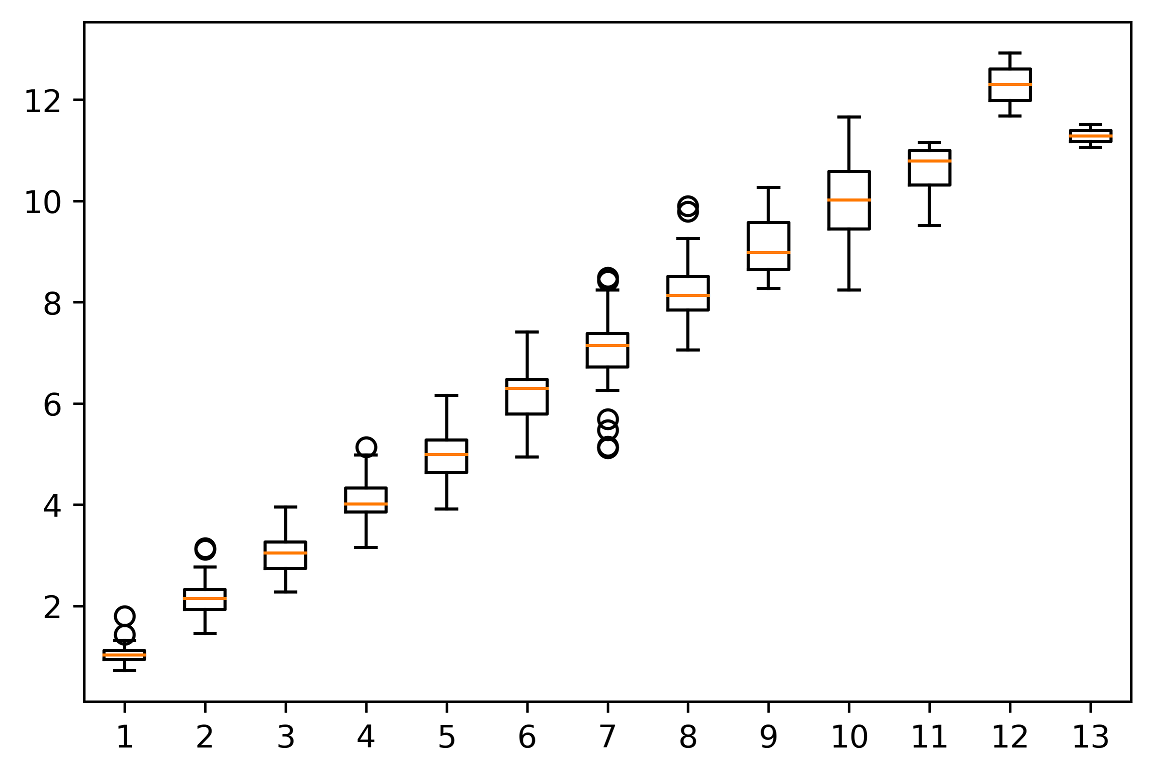
\includegraphics[width=0.5\textwidth]{result_pr_model/b4_min/boxplot_pr_age.png}}
  \subfloat[B4 minimum exposure residuals]{\label{ref_label2}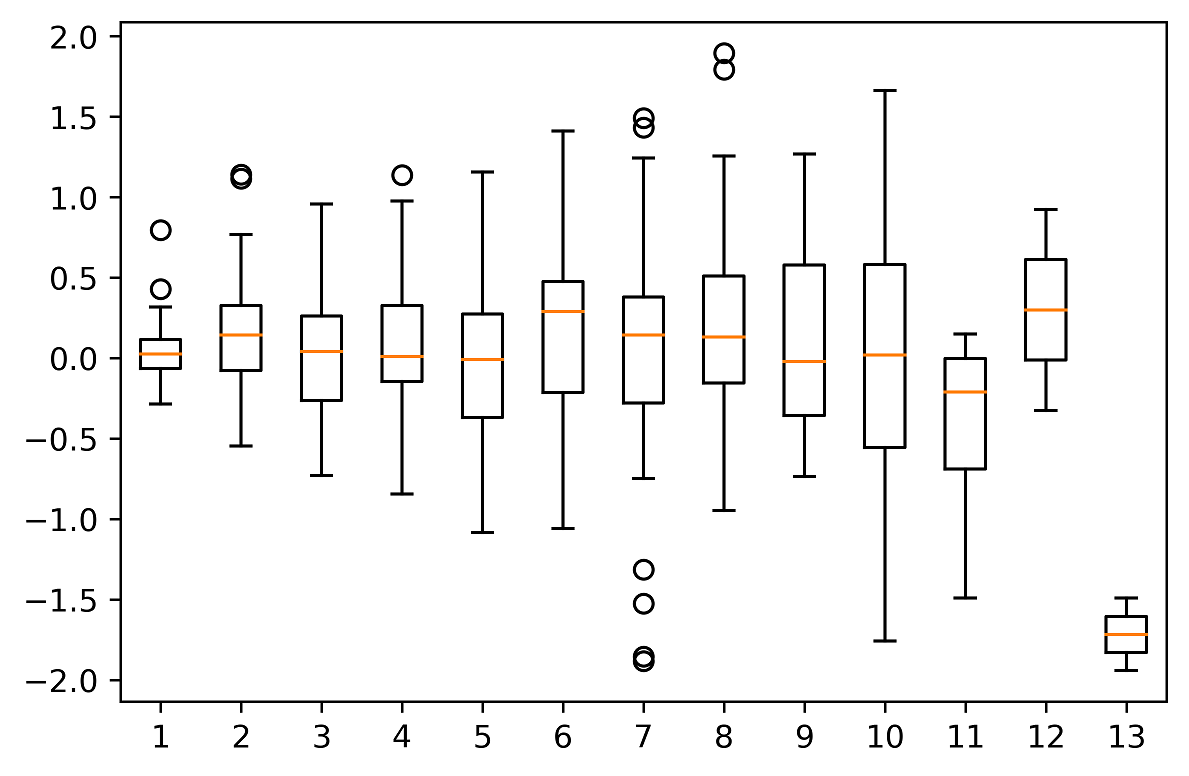
\includegraphics[width=0.5\textwidth]{result_pr_model/b4_min/boxplot_residual.png}}

  \subfloat[B5 minimum exposure]{\label{ref_label3}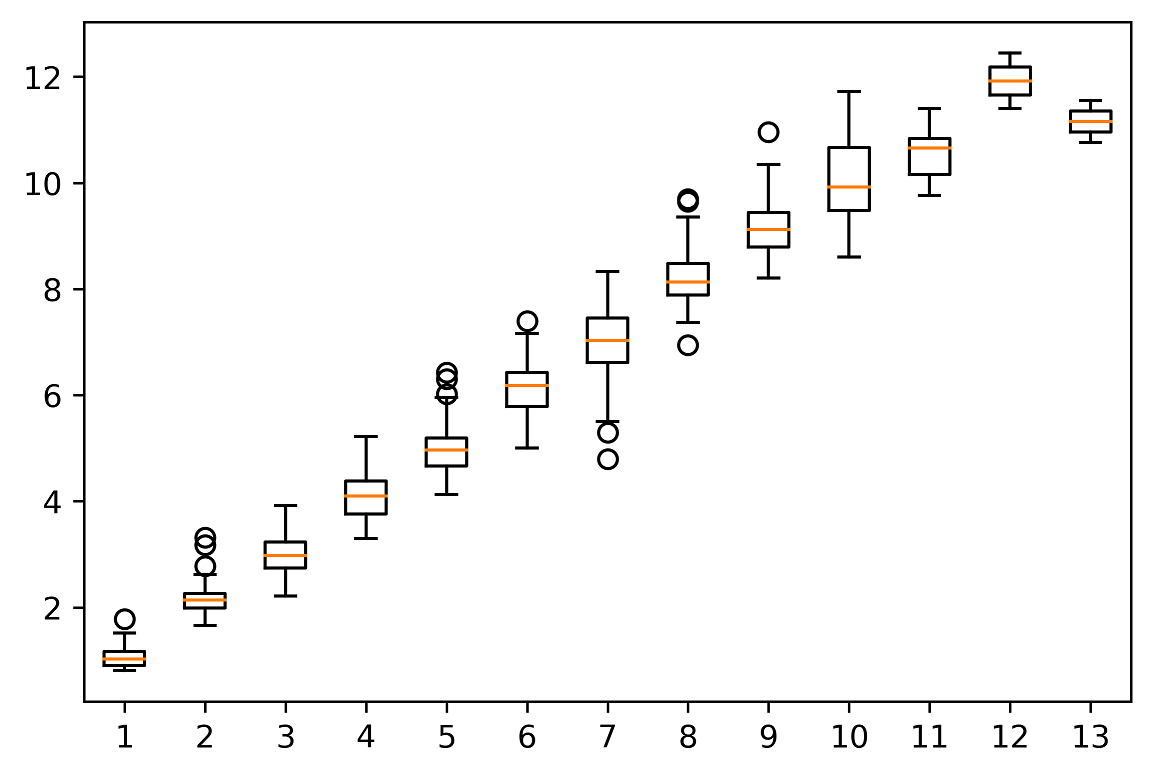
\includegraphics[width=0.5\textwidth]{result_pr_model/b5_min/boxplot_pr_age.png}}
  \subfloat[B5 minimum exposure, residuals]{\label{ref_label4}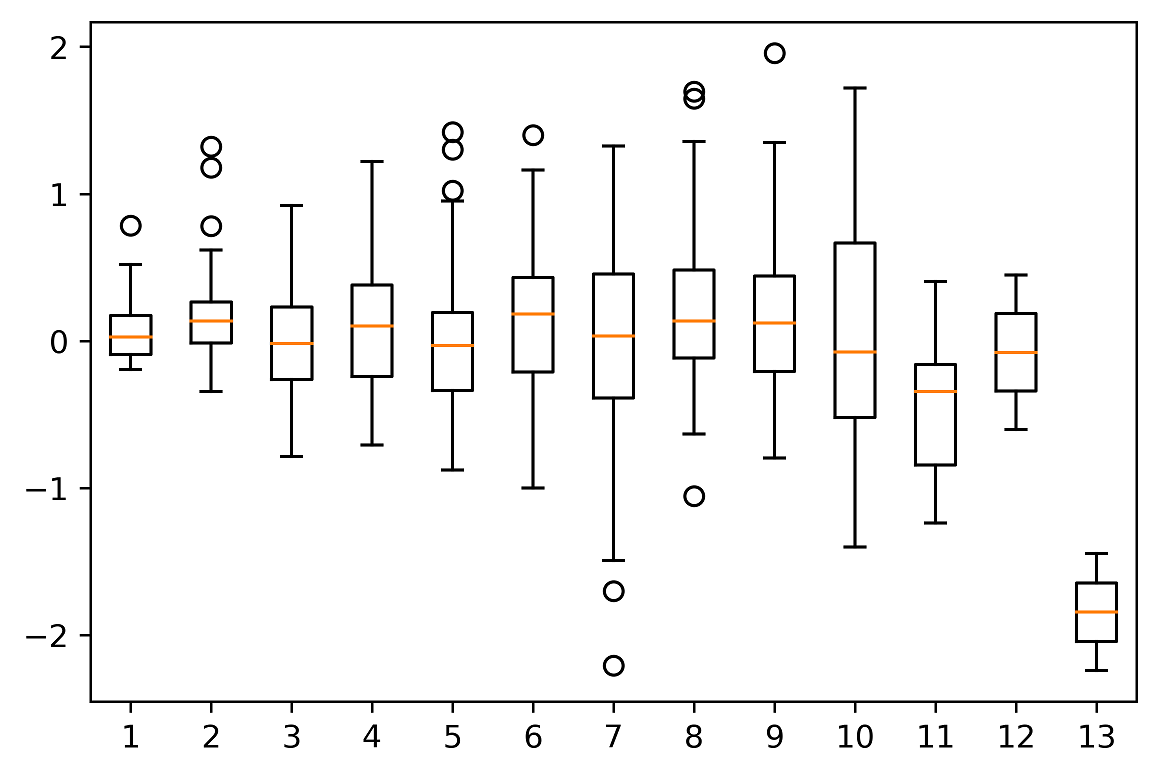
\includegraphics[width=0.5\textwidth]{result_pr_model/b5_min/boxplot_residual.png}}
  
  \subfloat[B6 minimum exposure]{\label{ref_label3}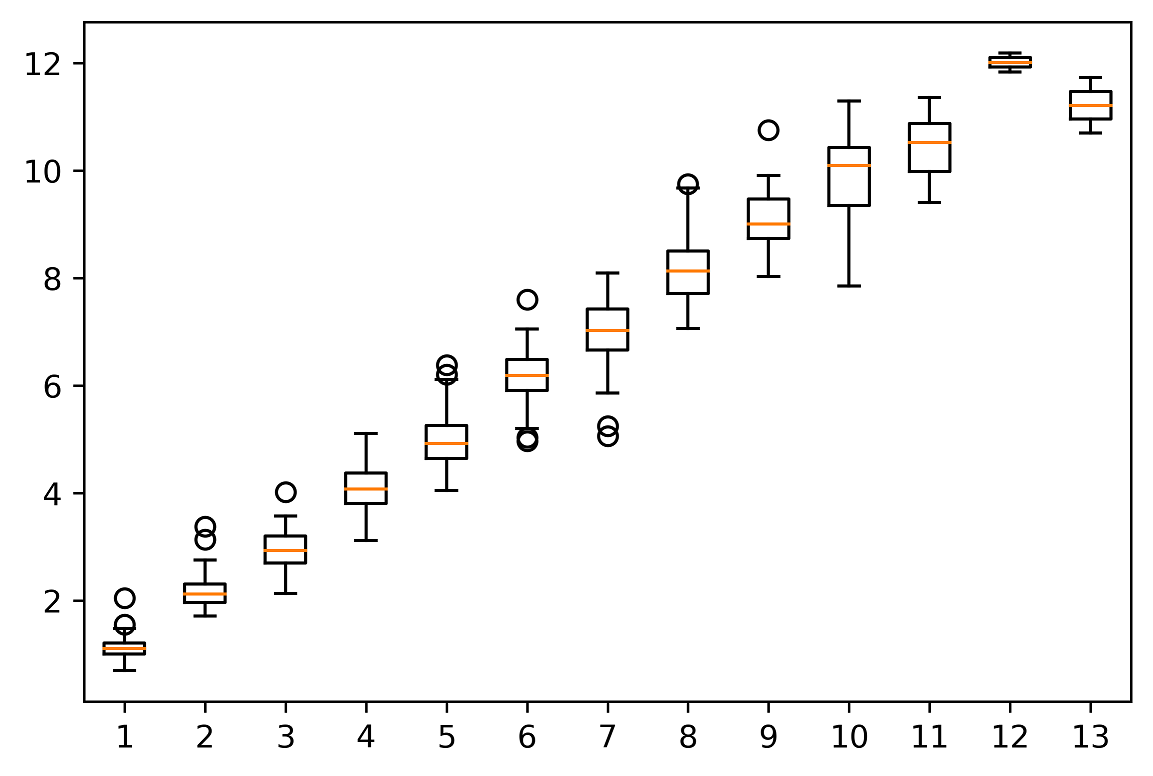
\includegraphics[width=0.5\textwidth]{result_pr_model/b6_min/boxplot_pr_age.png}}
  \subfloat[B6 minimum exposure, residuals]{\label{ref_label4}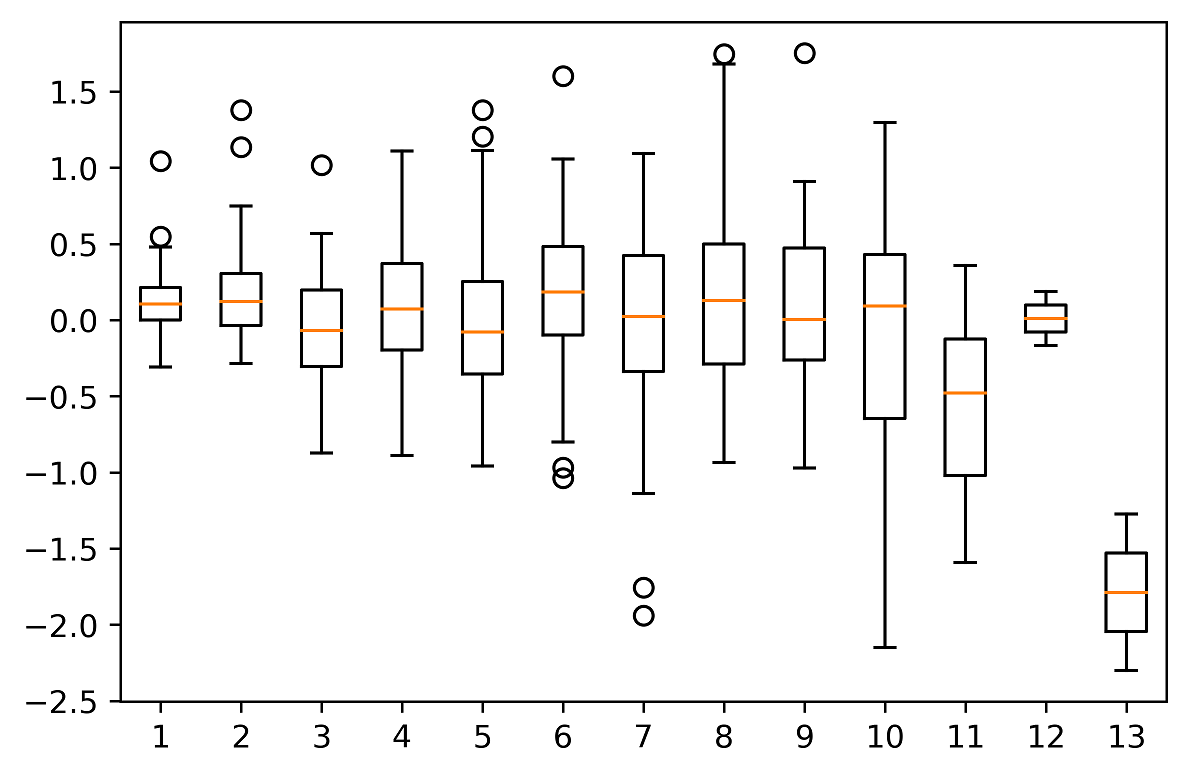
\includegraphics[width=0.5\textwidth]{result_pr_model/b6_min/boxplot_residual.png}}  
  \caption{\label{ref_label_overall}Comparing the models, looking at age per age class, and the residuals per prediction}
\end{figure}

Lets look at the scatter-plot of the errors which causes misclassifications.

\begin{figure}
  \centering
  \subfloat[B4 minimum exposure]{\label{ref_label1}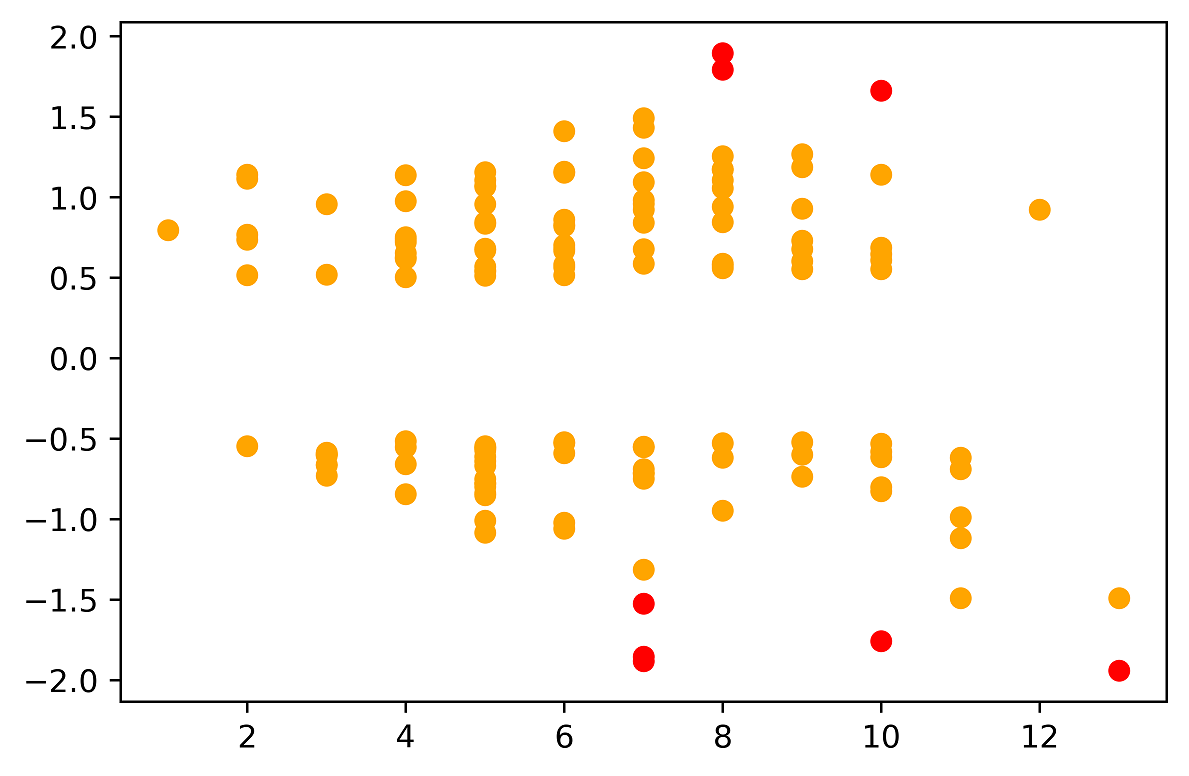
\includegraphics[width=0.5\textwidth]{result_pr_model/b4_min/misclassification.png}}

  \subfloat[B5 minimum exposure]{\label{ref_label3}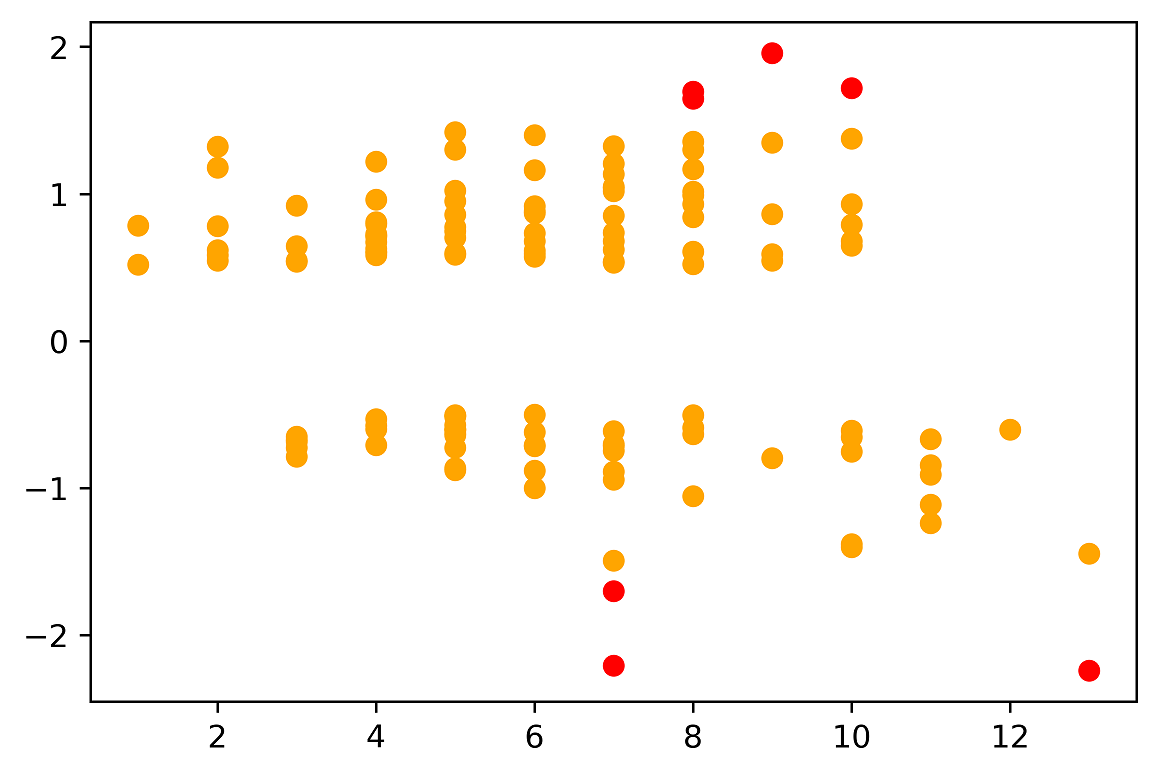
\includegraphics[width=0.5\textwidth]{result_pr_model/b5_min/misclassification.png}}
  
  \subfloat[B6 minimum exposure]{\label{ref_label3}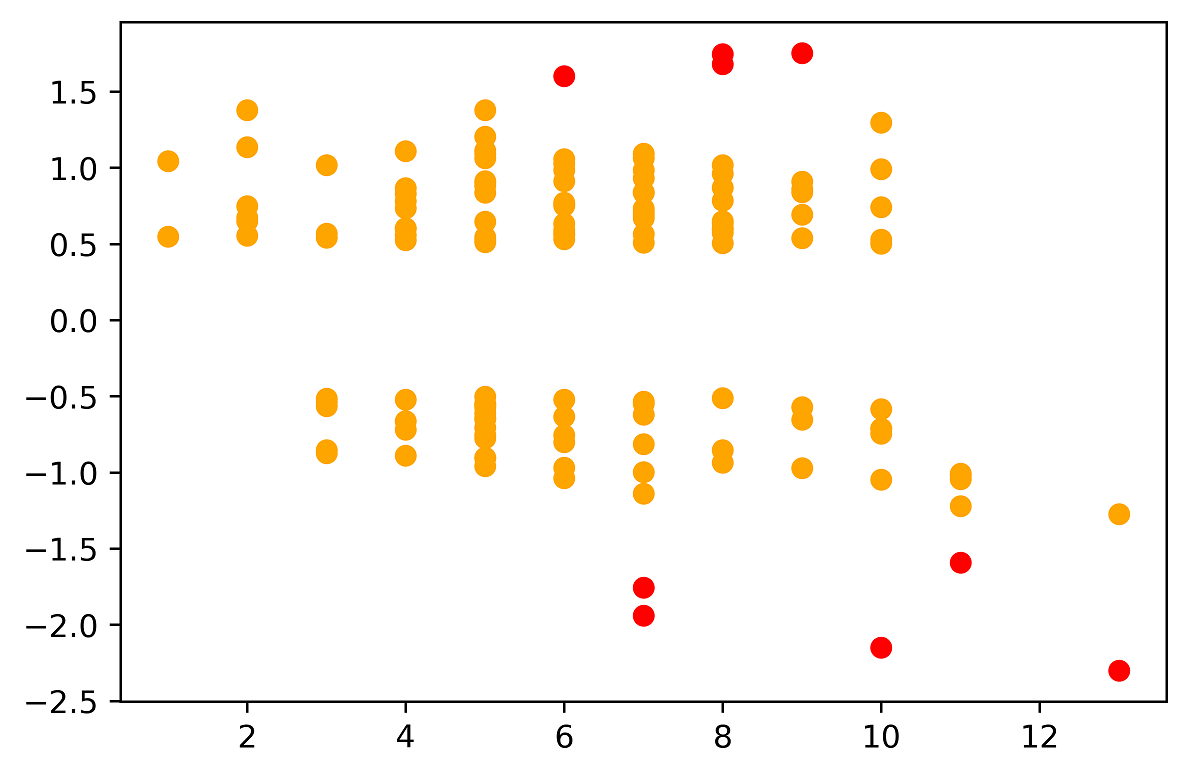
\includegraphics[width=0.5\textwidth]{result_pr_model/b6_min/misclassification.png}}
  \caption{\label{ref_label_overall}Comparing the models, looking at age per age class, and the reciduals per perdiction}
\end{figure}


\subsection*{Ensemble of ensembles}

We search the space of ensemble of ensemble predictions
which are given by 
$\sum_{k=1}^{N}\binom{N}{k} $ where $N=22$ and $k \in 1..N$

\begin{figure}[h!]
  \centering
  \begin{minipage}[b]{0.49\textwidth}
  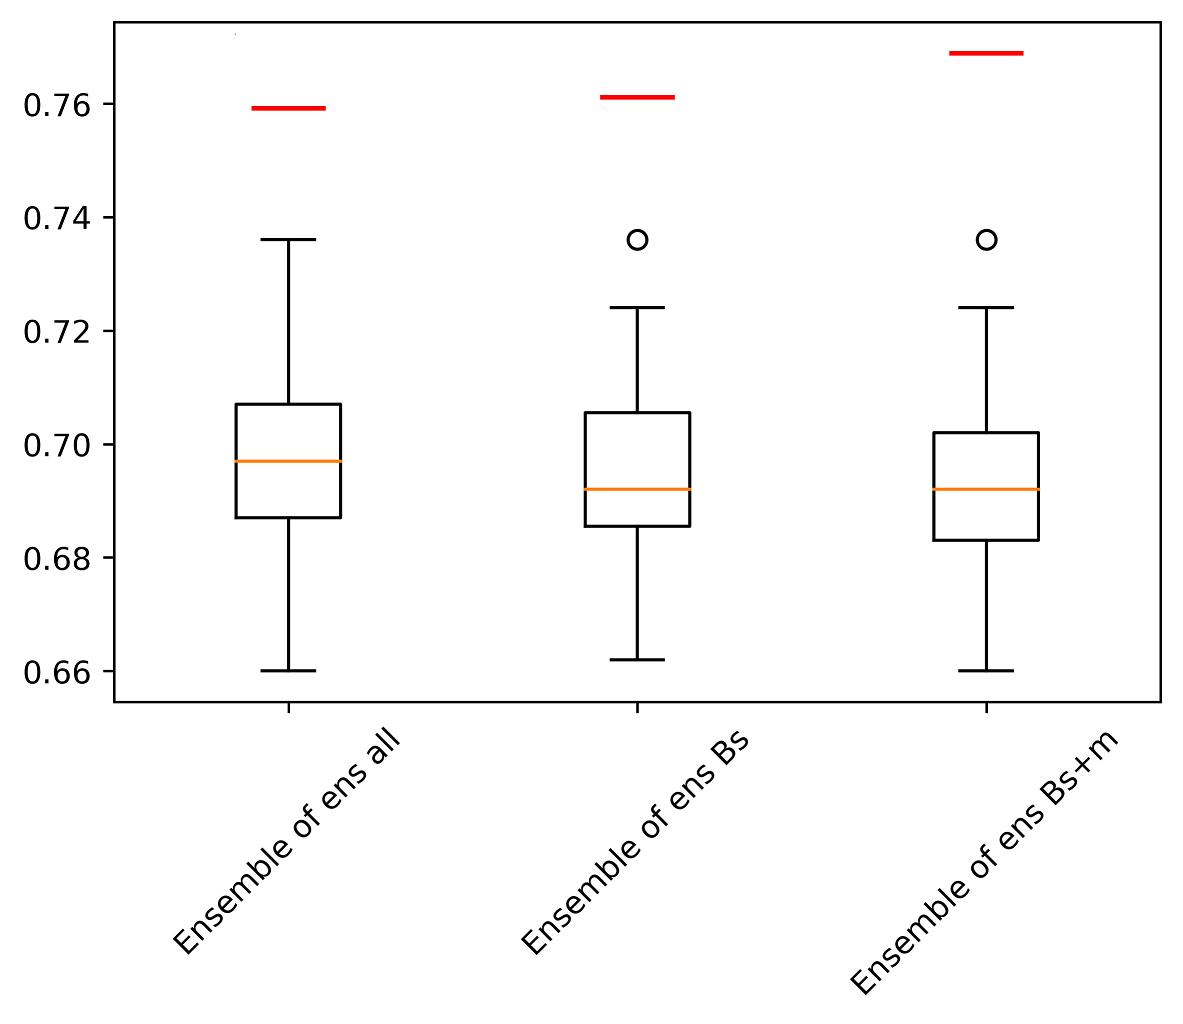
\includegraphics[scale=0.2]{results/eoe_acc.png}
    \caption{Ensemble of ensemble: accuracy of the 3 best models}
   \label{marker5}
  \end{minipage}
  \hfill
\end{figure}

\begin{figure}[h!]
  \centering
  \begin{minipage}[b]{0.49\textwidth}
  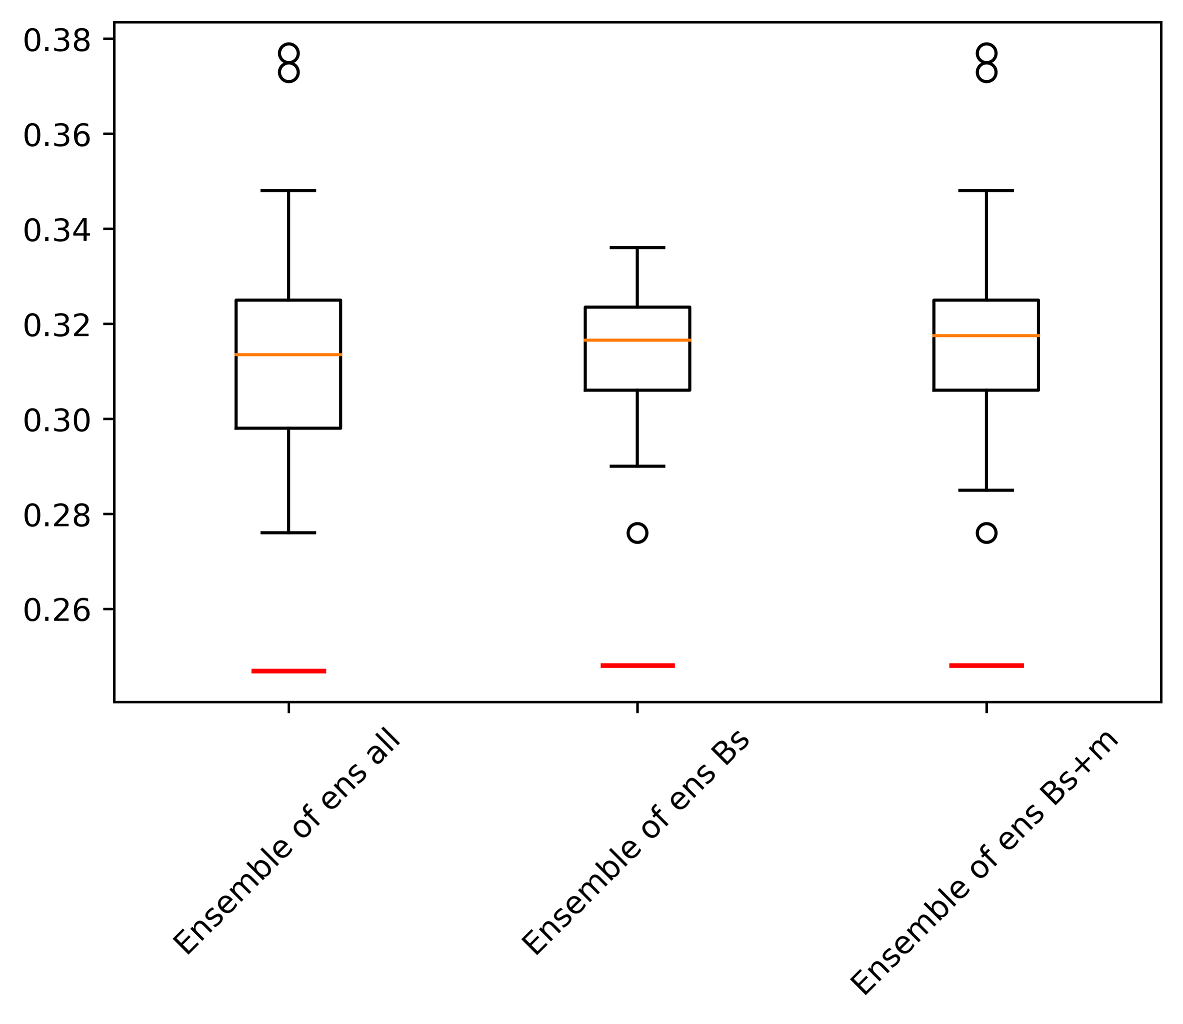
\includegraphics[scale=0.2]{results/eoe_mse.png}
    \caption{Ensemble of ensemble: mse of the 3 best models}
   \label{marker5}
  \end{minipage}
  \hfill
\end{figure}

\begin{center}
\begin{table}[hbt!]
\caption{Accuracy/MSE pr ensemble of ensemble.
Eoe1 is ensemble of ensemble of all models, Eoe2 is for B4, B5 and B6,
and Eoe3 is Eoe2 plus efficientNetV2 medium.}
\begin{tabular}{ |l|c|c|c| }
\hline
score/ensemble & eoe1 & eoe2 & eoe3  \\ \hline
Acc & 75.9 & 76.1 & 76.9 \\ 
MSE & .247 & .248 & .248  \\ 
\hline
\end{tabular}
\end{table}
\end{center}



\subsection*{Outliers}

Looking at figure (x) we can see that the model under predicts the age of older otoliths. This pattern is especially observable for individuals read as 15 years and older. The oldest predication is 18 years while the test set contains individuals as old as 22 years. To better understand the bias, figure \ref{marker5} shows the 4 largest outliers from the test set which come from two pairs

\begin{figure}[h!]
  \caption{The most common images miss predicted with more than 1.5 years}
  \centering
  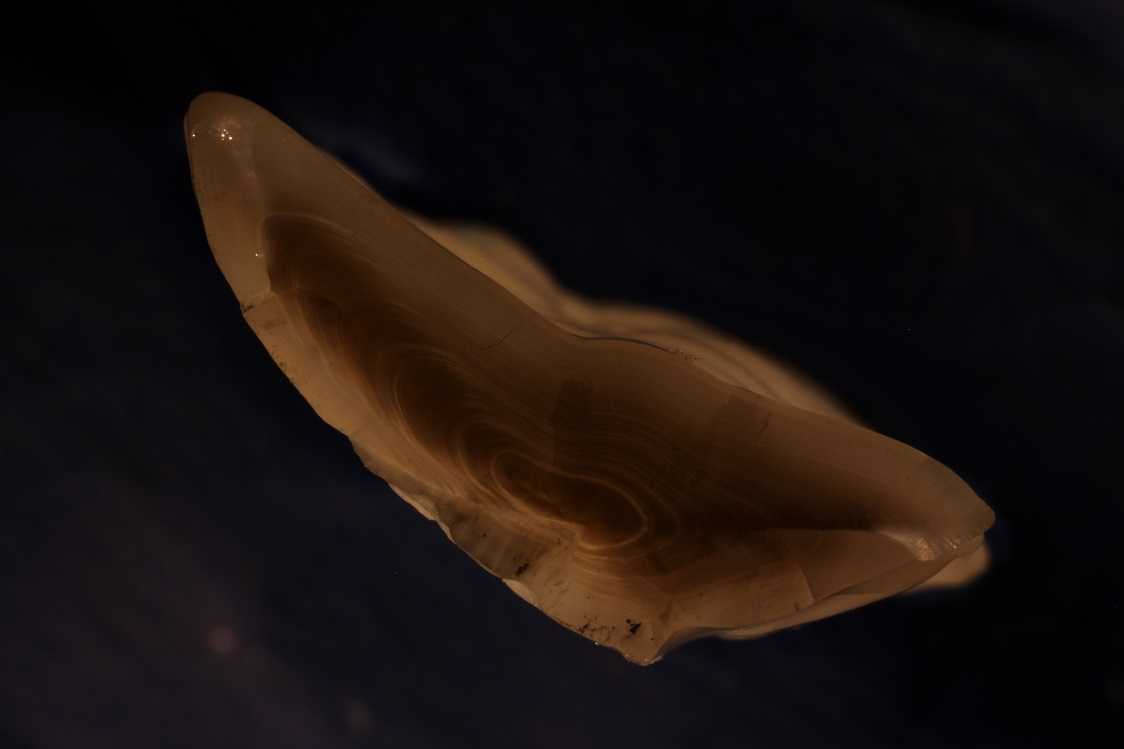
\includegraphics[scale=0.08]{outliers/IMG_0284_13.JPG}
  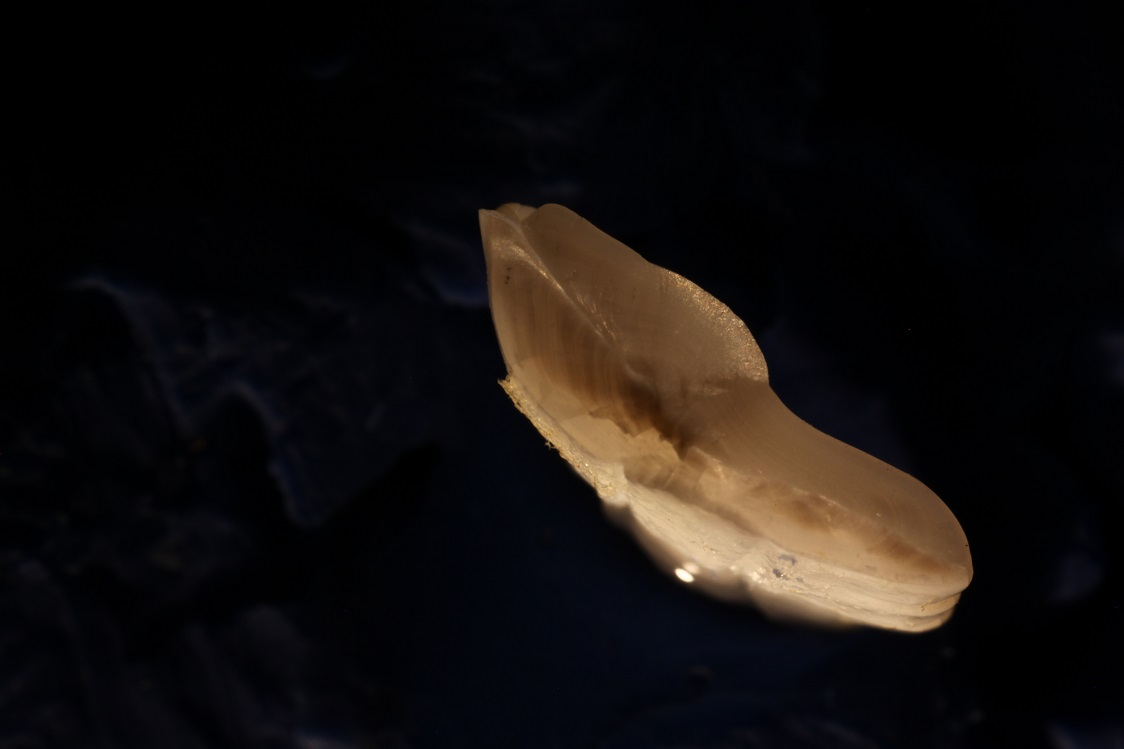
\includegraphics[scale=0.08]{outliers/IMG_0230_71.JPG}
  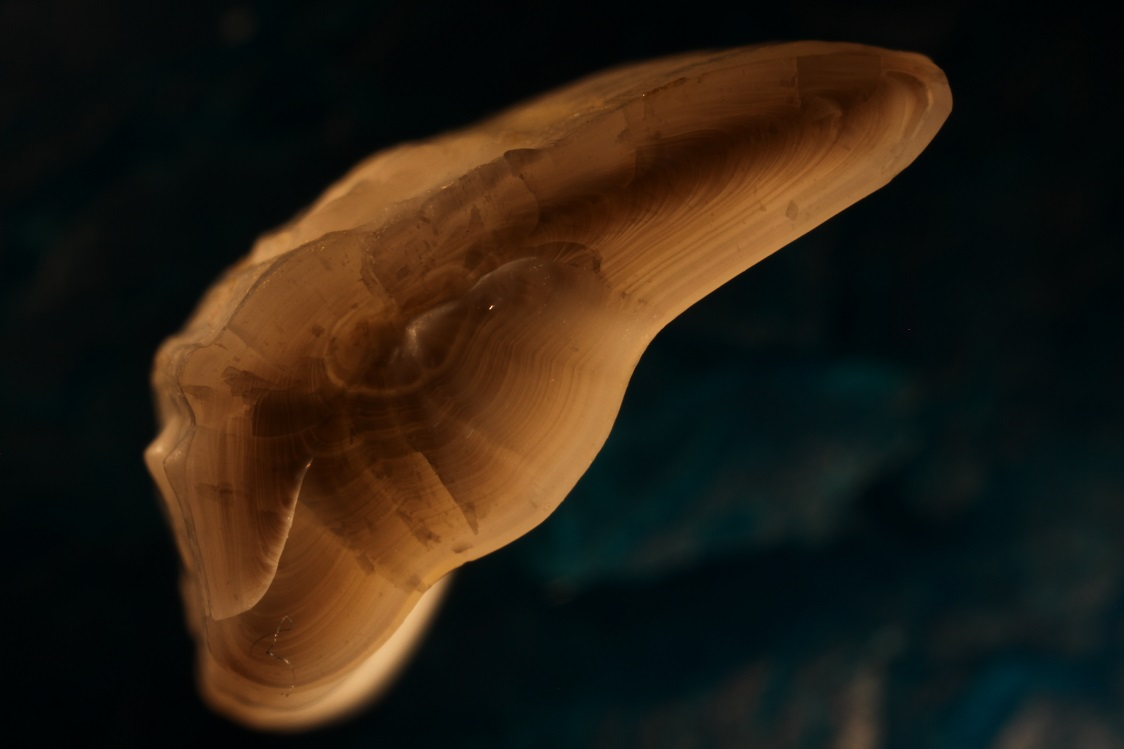
\includegraphics[scale=0.08]{outliers/IMG_0104_270.JPG} 

  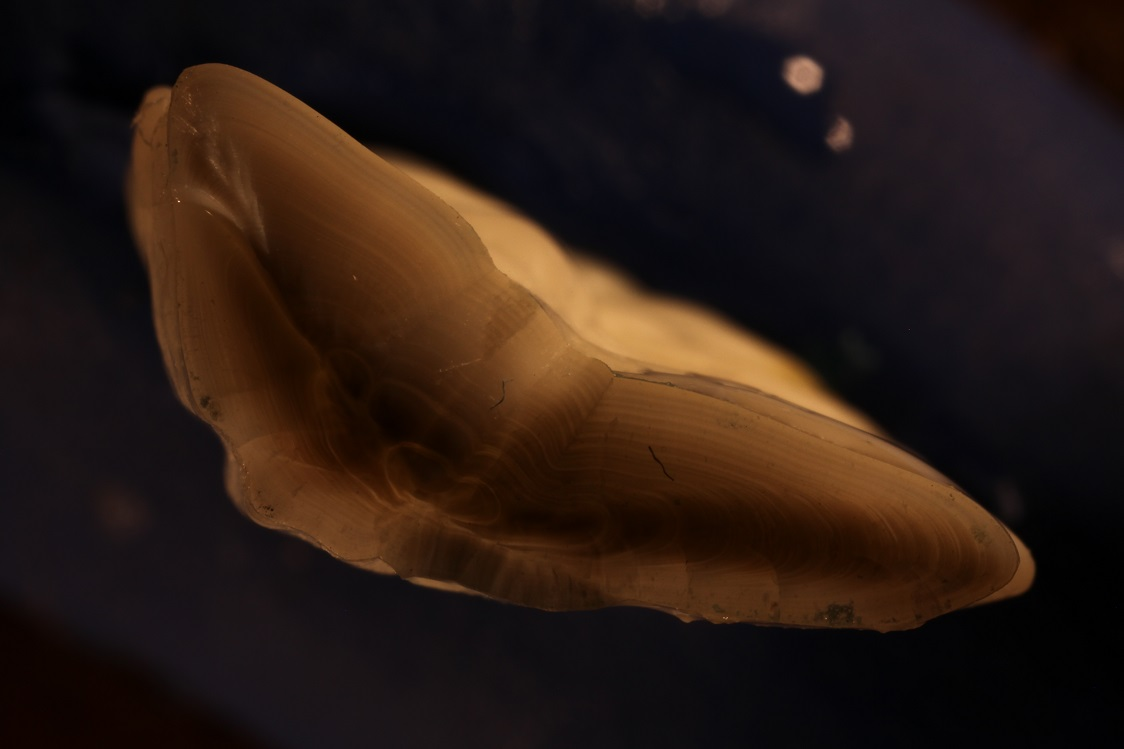
\includegraphics[scale=0.08]{outliers/IMG_0044_342.JPG}
  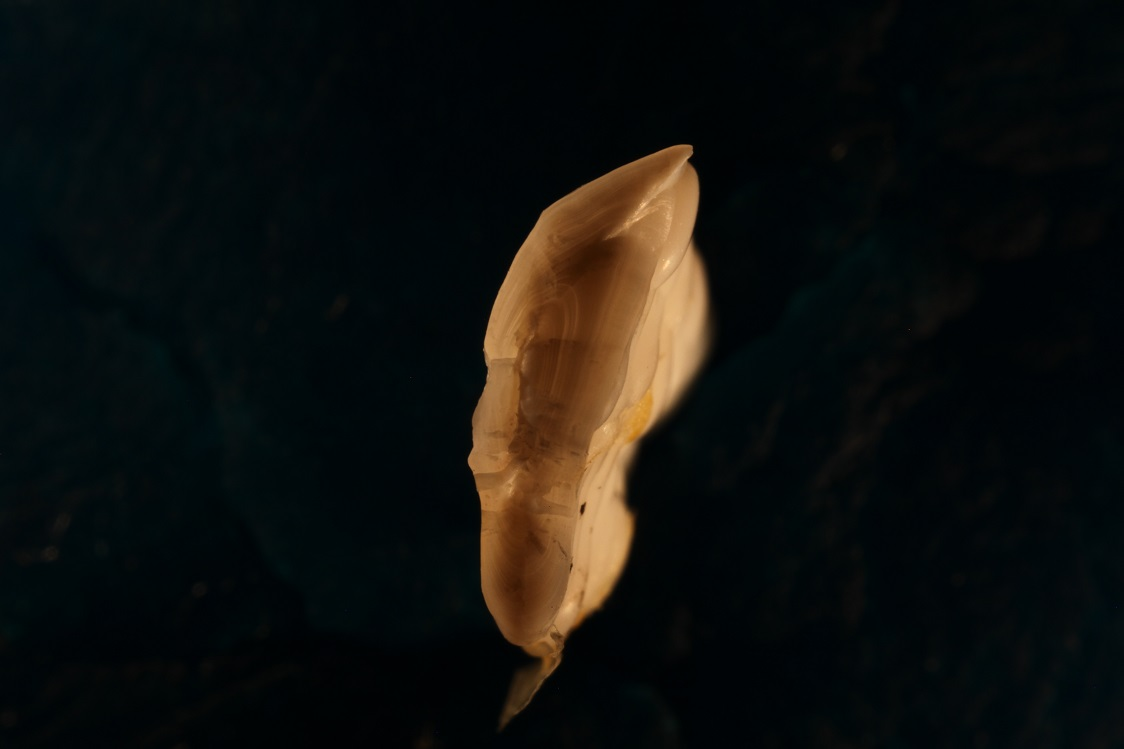
\includegraphics[scale=0.08]{outliers/IMG_0086_360.JPG}
  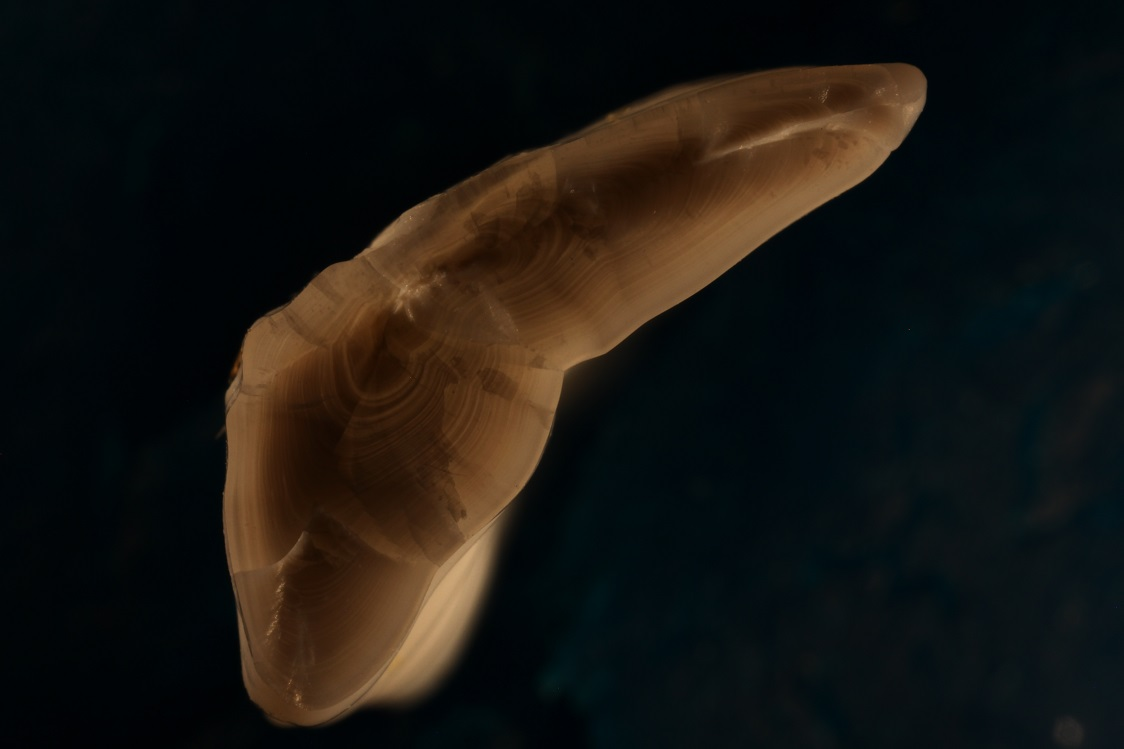
\includegraphics[scale=0.08]{outliers/IMG_0122_369.JPG}
  
  \label{marker10}
\end{figure}

Figure \ref{marker7} are the most commonly misclassified images 
with greatest magnitude of error.


\section*{Discussion}

During initial training we trained a B4 network on ca 2000 images and obtained
an accuracy of ca 60\%, later another 3000 images was added and the same
network was trained on ca 5000 images which resulted in accuracy of ca 70\%.
It could be interesting to investigating if adding another 3-5000 images
would increase the accuracy to 80\%.


\section*{References}

\bibliographystyle{apalike}
\bibliography{references}

\end{document}
